% Options for packages loaded elsewhere
\PassOptionsToPackage{unicode}{hyperref}
\PassOptionsToPackage{hyphens}{url}
%
\documentclass[
]{article}
\usepackage{lmodern}
\usepackage{amssymb,amsmath}
\usepackage{ifxetex,ifluatex}
\ifnum 0\ifxetex 1\fi\ifluatex 1\fi=0 % if pdftex
  \usepackage[T1]{fontenc}
  \usepackage[utf8]{inputenc}
  \usepackage{textcomp} % provide euro and other symbols
\else % if luatex or xetex
  \usepackage{unicode-math}
  \defaultfontfeatures{Scale=MatchLowercase}
  \defaultfontfeatures[\rmfamily]{Ligatures=TeX,Scale=1}
\fi
% Use upquote if available, for straight quotes in verbatim environments
\IfFileExists{upquote.sty}{\usepackage{upquote}}{}
\IfFileExists{microtype.sty}{% use microtype if available
  \usepackage[]{microtype}
  \UseMicrotypeSet[protrusion]{basicmath} % disable protrusion for tt fonts
}{}
\makeatletter
\@ifundefined{KOMAClassName}{% if non-KOMA class
  \IfFileExists{parskip.sty}{%
    \usepackage{parskip}
  }{% else
    \setlength{\parindent}{0pt}
    \setlength{\parskip}{6pt plus 2pt minus 1pt}}
}{% if KOMA class
  \KOMAoptions{parskip=half}}
\makeatother
\usepackage{xcolor}
\IfFileExists{xurl.sty}{\usepackage{xurl}}{} % add URL line breaks if available
\IfFileExists{bookmark.sty}{\usepackage{bookmark}}{\usepackage{hyperref}}
\hypersetup{
  pdftitle={Appendix},
  pdfauthor={Umberto Mignozzetti},
  hidelinks,
  pdfcreator={LaTeX via pandoc}}
\urlstyle{same} % disable monospaced font for URLs
\usepackage[margin=1in]{geometry}
\usepackage{color}
\usepackage{fancyvrb}
\newcommand{\VerbBar}{|}
\newcommand{\VERB}{\Verb[commandchars=\\\{\}]}
\DefineVerbatimEnvironment{Highlighting}{Verbatim}{commandchars=\\\{\}}
% Add ',fontsize=\small' for more characters per line
\usepackage{framed}
\definecolor{shadecolor}{RGB}{248,248,248}
\newenvironment{Shaded}{\begin{snugshade}}{\end{snugshade}}
\newcommand{\AlertTok}[1]{\textcolor[rgb]{0.94,0.16,0.16}{#1}}
\newcommand{\AnnotationTok}[1]{\textcolor[rgb]{0.56,0.35,0.01}{\textbf{\textit{#1}}}}
\newcommand{\AttributeTok}[1]{\textcolor[rgb]{0.77,0.63,0.00}{#1}}
\newcommand{\BaseNTok}[1]{\textcolor[rgb]{0.00,0.00,0.81}{#1}}
\newcommand{\BuiltInTok}[1]{#1}
\newcommand{\CharTok}[1]{\textcolor[rgb]{0.31,0.60,0.02}{#1}}
\newcommand{\CommentTok}[1]{\textcolor[rgb]{0.56,0.35,0.01}{\textit{#1}}}
\newcommand{\CommentVarTok}[1]{\textcolor[rgb]{0.56,0.35,0.01}{\textbf{\textit{#1}}}}
\newcommand{\ConstantTok}[1]{\textcolor[rgb]{0.00,0.00,0.00}{#1}}
\newcommand{\ControlFlowTok}[1]{\textcolor[rgb]{0.13,0.29,0.53}{\textbf{#1}}}
\newcommand{\DataTypeTok}[1]{\textcolor[rgb]{0.13,0.29,0.53}{#1}}
\newcommand{\DecValTok}[1]{\textcolor[rgb]{0.00,0.00,0.81}{#1}}
\newcommand{\DocumentationTok}[1]{\textcolor[rgb]{0.56,0.35,0.01}{\textbf{\textit{#1}}}}
\newcommand{\ErrorTok}[1]{\textcolor[rgb]{0.64,0.00,0.00}{\textbf{#1}}}
\newcommand{\ExtensionTok}[1]{#1}
\newcommand{\FloatTok}[1]{\textcolor[rgb]{0.00,0.00,0.81}{#1}}
\newcommand{\FunctionTok}[1]{\textcolor[rgb]{0.00,0.00,0.00}{#1}}
\newcommand{\ImportTok}[1]{#1}
\newcommand{\InformationTok}[1]{\textcolor[rgb]{0.56,0.35,0.01}{\textbf{\textit{#1}}}}
\newcommand{\KeywordTok}[1]{\textcolor[rgb]{0.13,0.29,0.53}{\textbf{#1}}}
\newcommand{\NormalTok}[1]{#1}
\newcommand{\OperatorTok}[1]{\textcolor[rgb]{0.81,0.36,0.00}{\textbf{#1}}}
\newcommand{\OtherTok}[1]{\textcolor[rgb]{0.56,0.35,0.01}{#1}}
\newcommand{\PreprocessorTok}[1]{\textcolor[rgb]{0.56,0.35,0.01}{\textit{#1}}}
\newcommand{\RegionMarkerTok}[1]{#1}
\newcommand{\SpecialCharTok}[1]{\textcolor[rgb]{0.00,0.00,0.00}{#1}}
\newcommand{\SpecialStringTok}[1]{\textcolor[rgb]{0.31,0.60,0.02}{#1}}
\newcommand{\StringTok}[1]{\textcolor[rgb]{0.31,0.60,0.02}{#1}}
\newcommand{\VariableTok}[1]{\textcolor[rgb]{0.00,0.00,0.00}{#1}}
\newcommand{\VerbatimStringTok}[1]{\textcolor[rgb]{0.31,0.60,0.02}{#1}}
\newcommand{\WarningTok}[1]{\textcolor[rgb]{0.56,0.35,0.01}{\textbf{\textit{#1}}}}
\usepackage{graphicx,grffile}
\makeatletter
\def\maxwidth{\ifdim\Gin@nat@width>\linewidth\linewidth\else\Gin@nat@width\fi}
\def\maxheight{\ifdim\Gin@nat@height>\textheight\textheight\else\Gin@nat@height\fi}
\makeatother
% Scale images if necessary, so that they will not overflow the page
% margins by default, and it is still possible to overwrite the defaults
% using explicit options in \includegraphics[width, height, ...]{}
\setkeys{Gin}{width=\maxwidth,height=\maxheight,keepaspectratio}
% Set default figure placement to htbp
\makeatletter
\def\fps@figure{htbp}
\makeatother
\setlength{\emergencystretch}{3em} % prevent overfull lines
\providecommand{\tightlist}{%
  \setlength{\itemsep}{0pt}\setlength{\parskip}{0pt}}
\setcounter{secnumdepth}{-\maxdimen} % remove section numbering
\usepackage{booktabs}
\usepackage{longtable}
\usepackage{array}
\usepackage{multirow}
\usepackage{wrapfig}
\usepackage{float}
\usepackage{colortbl}
\usepackage{pdflscape}
\usepackage{tabu}
\usepackage{threeparttable}
\usepackage{threeparttablex}
\usepackage[normalem]{ulem}
\usepackage{makecell}
\usepackage{xcolor}

\title{Appendix}
\author{Umberto Mignozzetti}
\date{12/25/2019}

\begin{document}
\maketitle

\tableofcontents

\hypertarget{search-criteria}{%
\subsection{Search criteria}\label{search-criteria}}

\hypertarget{search-terms}{%
\subsubsection{Search terms}\label{search-terms}}

XXXX

\hypertarget{searched-databases}{%
\subsubsection{Searched databases}\label{searched-databases}}

XXXX To Catarina: name and URL of database searched

\hypertarget{summary-total-results}{%
\subsubsection{Summary total results}\label{summary-total-results}}

XXXX To Catarina: put here results per database, cross-matching,
anything else

\hypertarget{exclusion-criteria}{%
\subsubsection{Exclusion criteria}\label{exclusion-criteria}}

\hypertarget{exclusion-title-and-abstract}{%
\paragraph{Exclusion title and
abstract}\label{exclusion-title-and-abstract}}

XXXX To Catarina: what criteria for first round exclusions?

\hypertarget{exclusion-reading}{%
\paragraph{Exclusion reading}\label{exclusion-reading}}

XXXX To Catarina: criteria second round exclusions

\hypertarget{exclusion-analysis}{%
\paragraph{Exclusion analysis}\label{exclusion-analysis}}

For the articles that passed the first two filters, we looked into the
tables and the reported coefficients. We kept articles in this step
based on two criteria:

\begin{enumerate}
\def\labelenumi{\arabic{enumi}.}
\tightlist
\item
  Matched treatment variable:
\end{enumerate}

\begin{itemize}
\tightlist
\item
  N: Number Legislators Lower House
\item
  logN: Log Number Legislators Lower House
\item
  K: Number Legislators Upper House
\end{itemize}

\begin{enumerate}
\def\labelenumi{\arabic{enumi}.}
\setcounter{enumi}{1}
\tightlist
\item
  Matched outcome variable:
\end{enumerate}

\begin{itemize}
\tightlist
\item
  ExpPC: Expenditure Per Capita
\item
  logExpPC: Log Expenditure Per Capita
\item
  PCTGDP: Percent GDP Public Expenditure
\end{itemize}

\hypertarget{prism}{%
\subsubsection{PRISM}\label{prism}}

\begin{itemize}
\tightlist
\item
  Number of articles matching the search criteria: XXXX
\item
  Number of articles excluded after title and abstract: XXXX
\item
  Number of articles excluded after reading: XXXX
\item
  Number of articles excluded before analysis: 3
\item
  Number of articles excluded during the analysis: 0
\end{itemize}

We have 26 articles in the meta-analysis.

\hypertarget{meta-analysis-dataset}{%
\subsection{Meta-analysis dataset}\label{meta-analysis-dataset}}

The meta-analytic data is comprised of two datasets. The first dataset
has the main coefficients that were reported in the paper. XXXX (Copiar
da parte de métodos).

\hypertarget{adding-articles}{%
\subsection{Adding articles}\label{adding-articles}}

\newpage

\hypertarget{descriptive-statistics}{%
\subsection{Descriptive statistics}\label{descriptive-statistics}}

\hypertarget{study-year}{%
\subsubsection{Study Year}\label{study-year}}

\begin{figure}
\centering
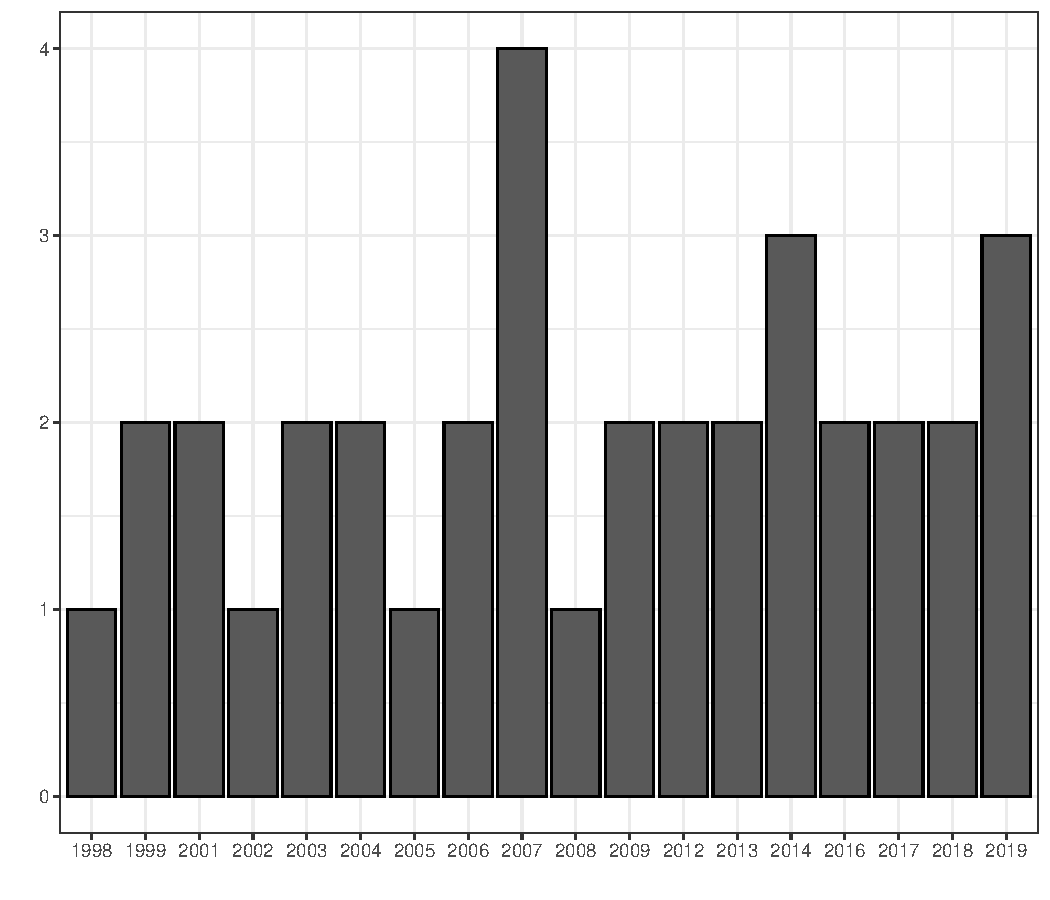
\includegraphics{appendixV5_files/figure-latex/unnamed-chunk-2-1.pdf}
\caption{Study Year Frequencies}
\end{figure}

\newpage

\hypertarget{published}{%
\subsubsection{Published?}\label{published}}

\begin{figure}
\centering
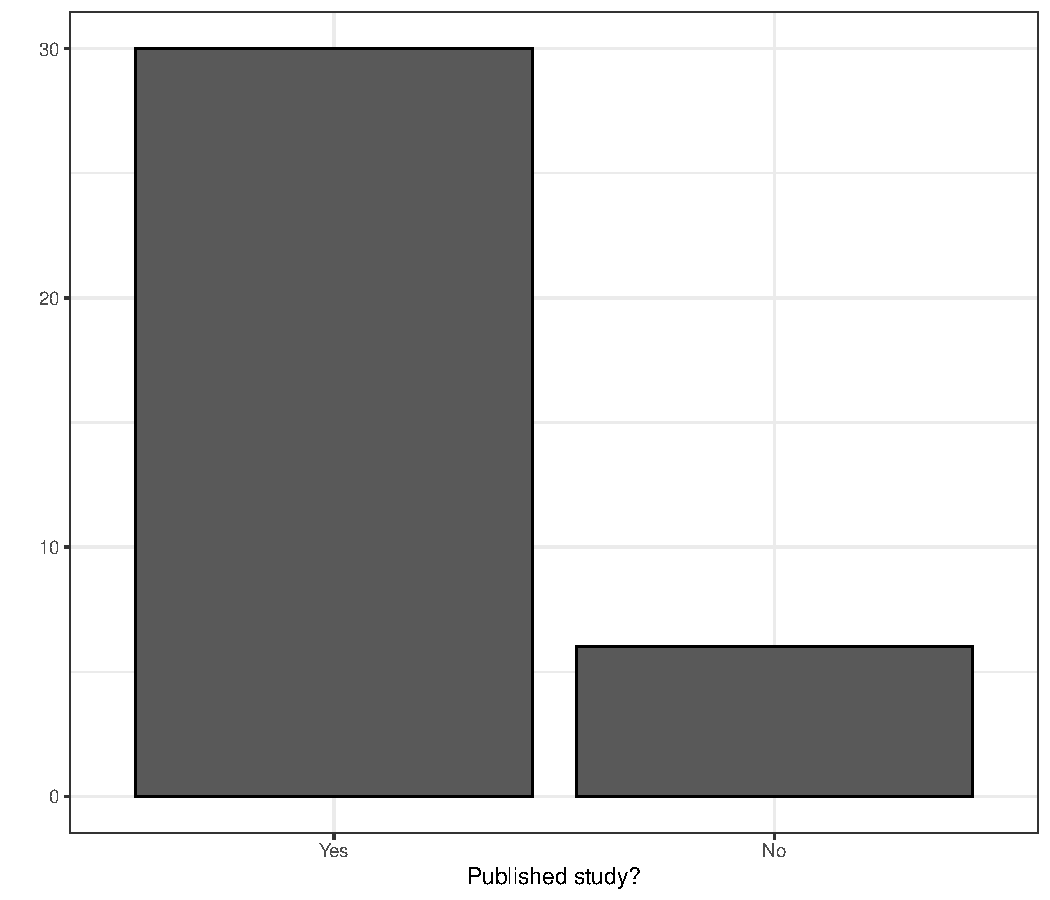
\includegraphics{appendixV5_files/figure-latex/unnamed-chunk-3-1.pdf}
\caption{Was the study published?}
\end{figure}

\newpage

\hypertarget{dependent-variables}{%
\subsubsection{Dependent variables}\label{dependent-variables}}

\begin{figure}
\centering
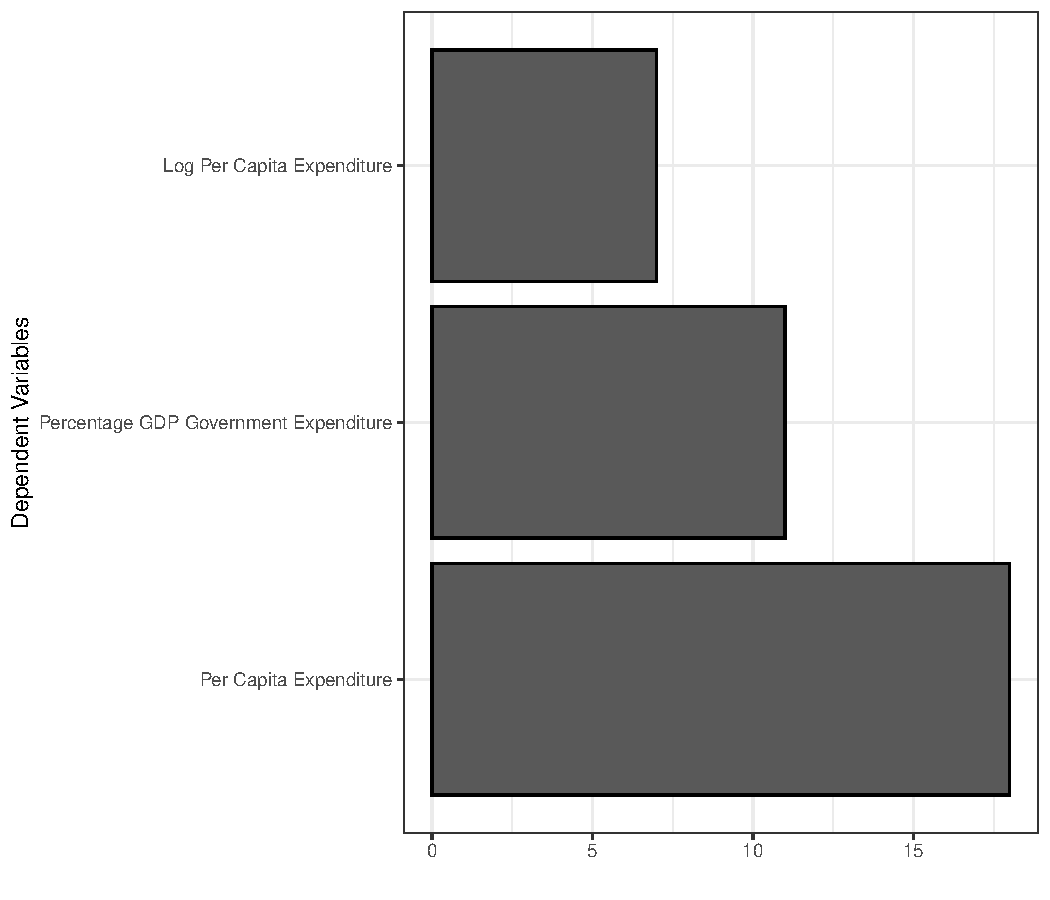
\includegraphics{appendixV5_files/figure-latex/unnamed-chunk-4-1.pdf}
\caption{Dependent variables across the law of 1/n studies}
\end{figure}

\newpage

\hypertarget{independent-variables}{%
\subsubsection{Independent variables}\label{independent-variables}}

\begin{figure}
\centering
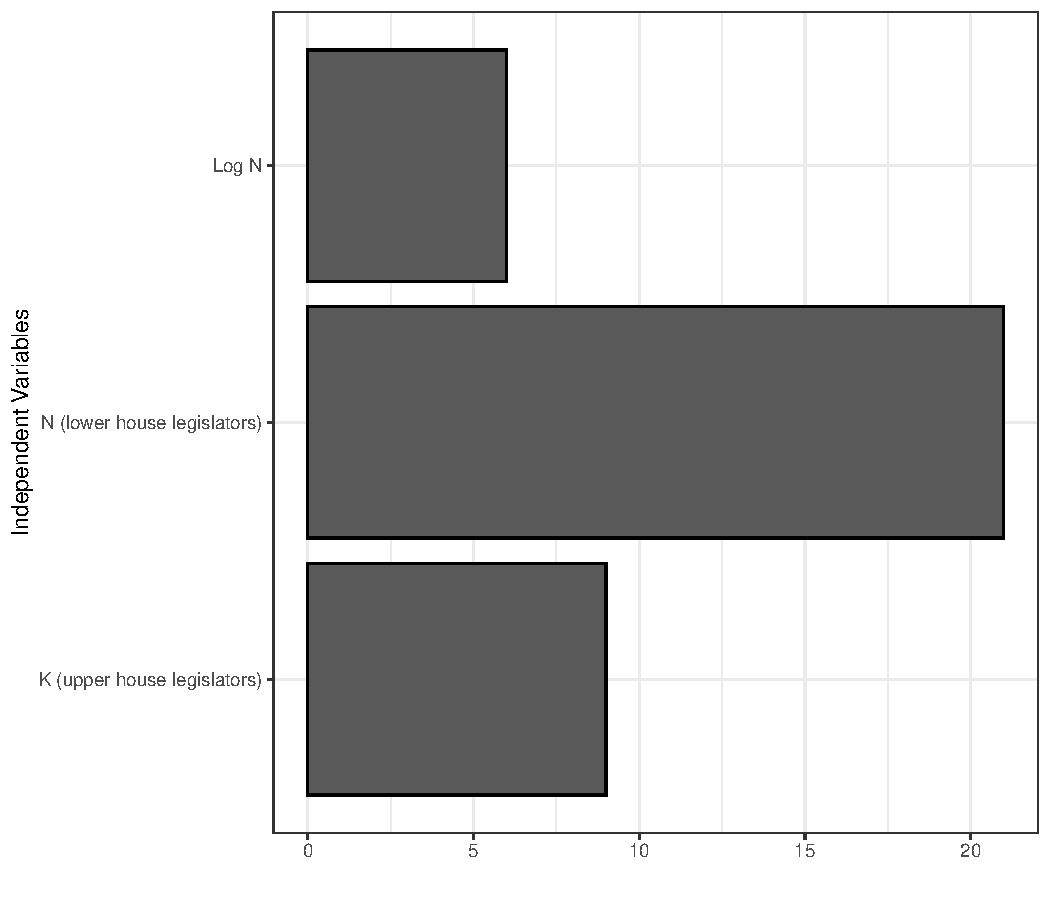
\includegraphics{appendixV5_files/figure-latex/unnamed-chunk-5-1.pdf}
\caption{Independent variables across the law of 1/n studies}
\end{figure}

\newpage

\hypertarget{histogram-coefficients}{%
\subsubsection{Histogram Coefficients}\label{histogram-coefficients}}

\begin{figure}
\centering
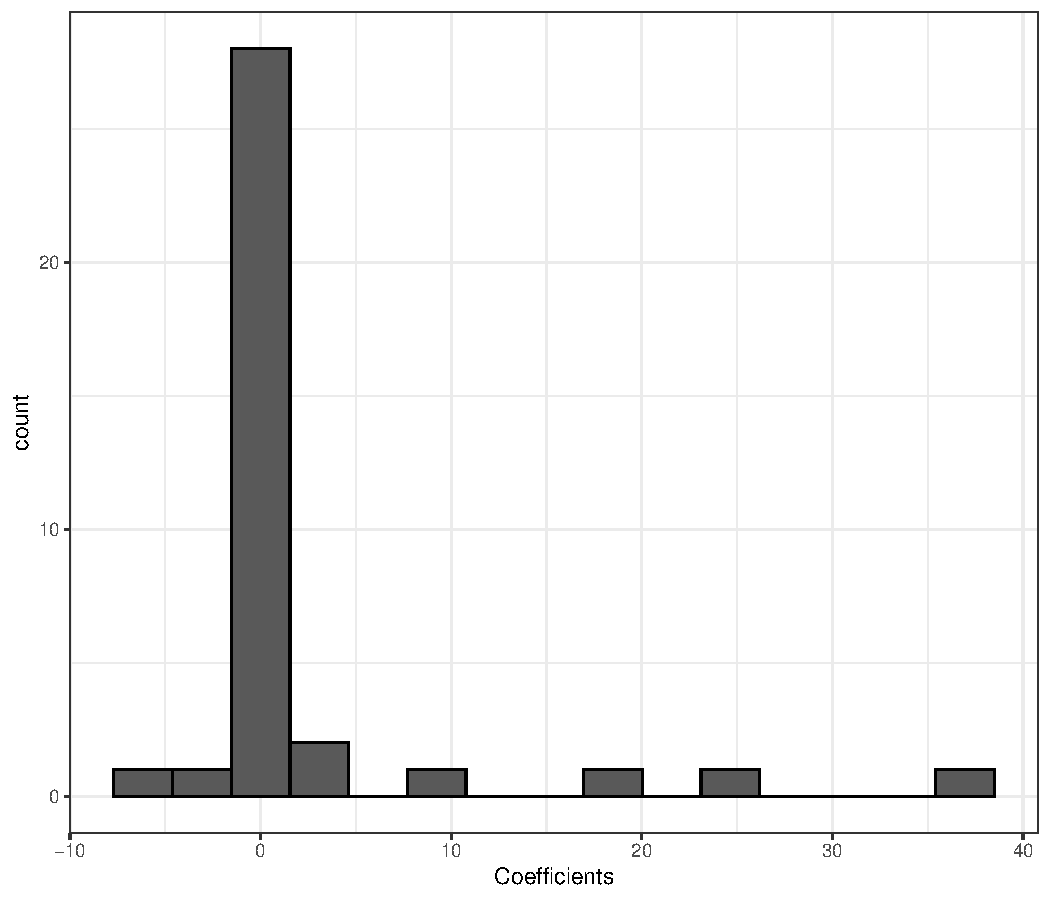
\includegraphics{appendixV5_files/figure-latex/unnamed-chunk-6-1.pdf}
\caption{Histogram Coefficients}
\end{figure}

\newpage

\hypertarget{histogram-standard-errors}{%
\subsubsection{Histogram Standard
Errors}\label{histogram-standard-errors}}

\begin{figure}
\centering
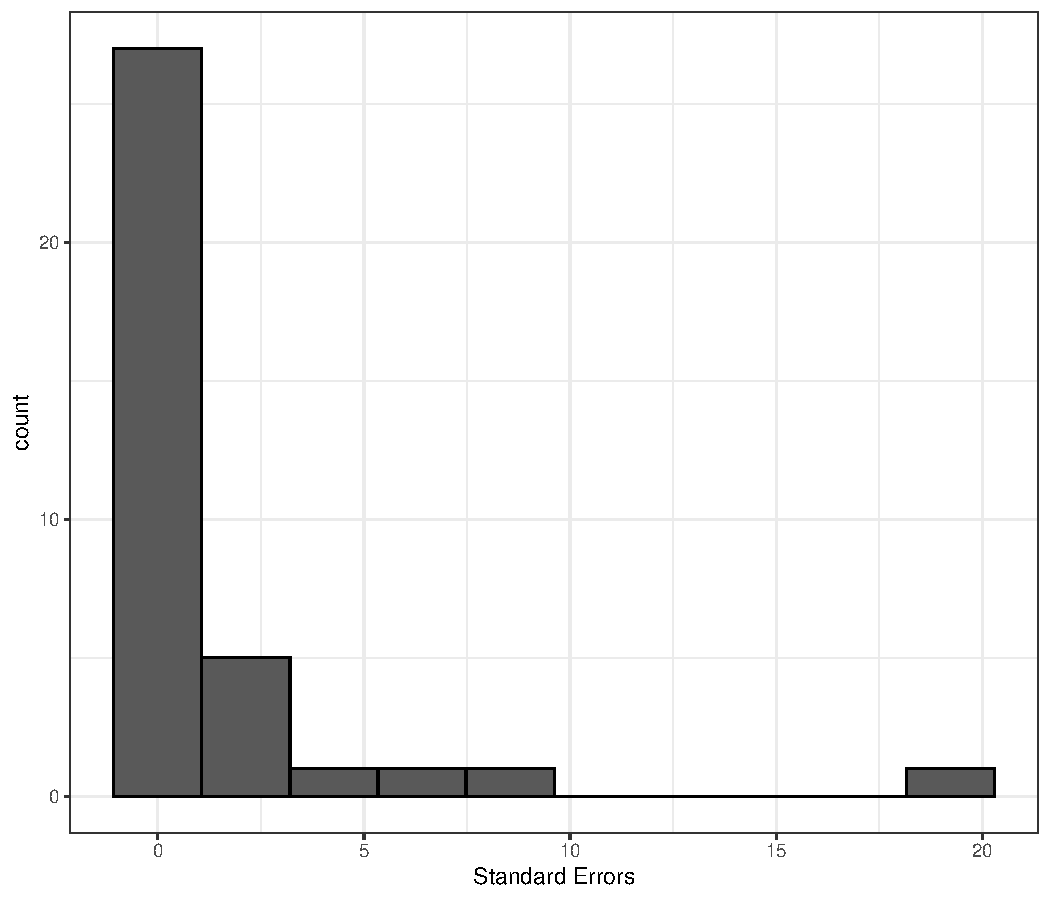
\includegraphics{appendixV5_files/figure-latex/unnamed-chunk-7-1.pdf}
\caption{Histogram Standard Errors}
\end{figure}

\newpage

\hypertarget{sign-coefficients}{%
\subsubsection{Sign Coefficients}\label{sign-coefficients}}

\begin{figure}
\centering
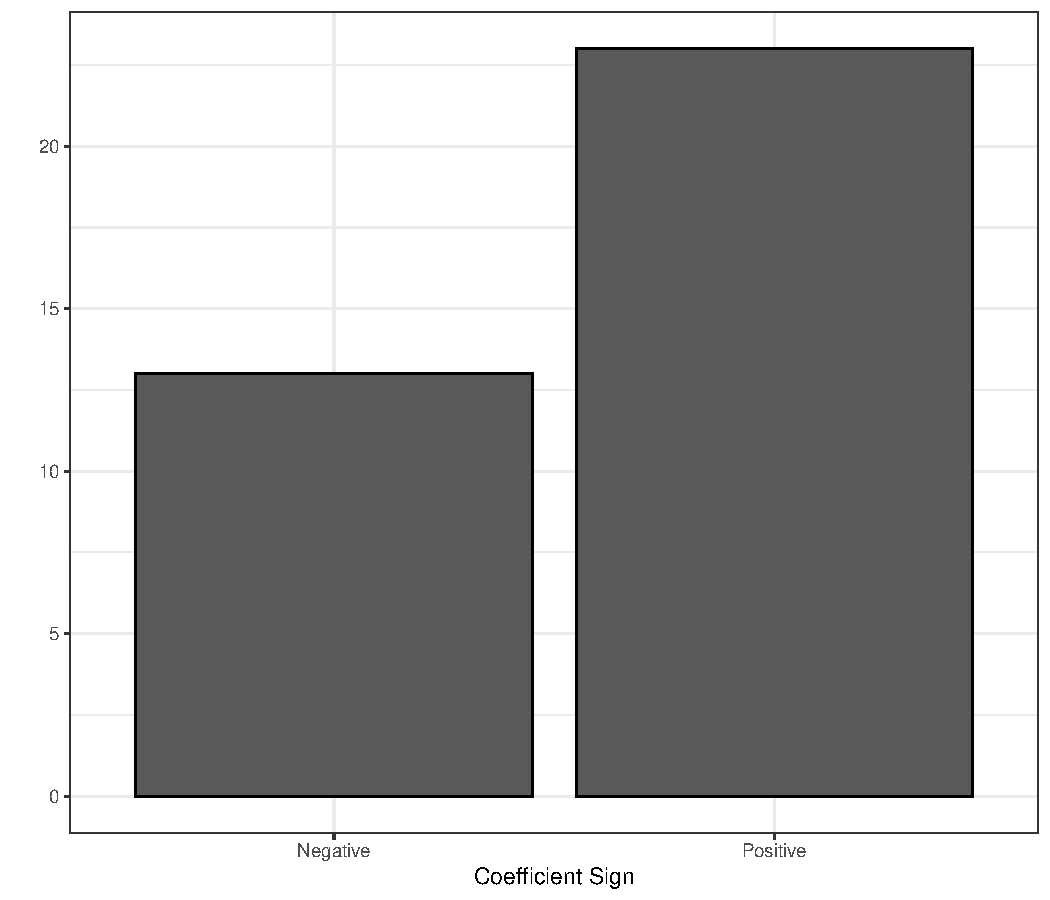
\includegraphics{appendixV5_files/figure-latex/unnamed-chunk-8-1.pdf}
\caption{Coefficient Sign?}
\end{figure}

A general test of the theory would be to study whether the coefficients
are positive or negative. Note that the law of 1/n would pose that we
should have a positive influence of legislature size on expenditure. To
test this theory, we run a Binomial One-Proportion Z-test. For the
number of legislators in the lower house (N), the results follow below.

\begin{verbatim}
## 
##  Exact binomial test
## 
## data:  table(aux$scoef)[1] and sum(table(aux$scoef))
## number of successes = 11, number of trials = 21, p-value = 1
## alternative hypothesis: true probability of success is not equal to 0.5
## 95 percent confidence interval:
##  0.2978068 0.7428694
## sample estimates:
## probability of success 
##              0.5238095
\end{verbatim}

Therefore, the most elementary test we could run, a sign direction test,
tells us that the law of 1/n does not hold for our sample. For the
number of legislators in the upper house (K), the results follow below.

\begin{verbatim}
## 
##  Exact binomial test
## 
## data:  table(aux$scoef)[1] and sum(table(aux$scoef))
## number of successes = 1, number of trials = 9, p-value = 0.03906
## alternative hypothesis: true probability of success is not equal to 0.5
## 95 percent confidence interval:
##  0.002809137 0.482496515
## sample estimates:
## probability of success 
##              0.1111111
\end{verbatim}

Here, the law of 1/n holds. However, the effect goes in a direction
different from the predicted in the law of k/n paper.

\newpage

\hypertarget{electoral-system}{%
\subsubsection{Electoral system}\label{electoral-system}}

\begin{figure}
\centering
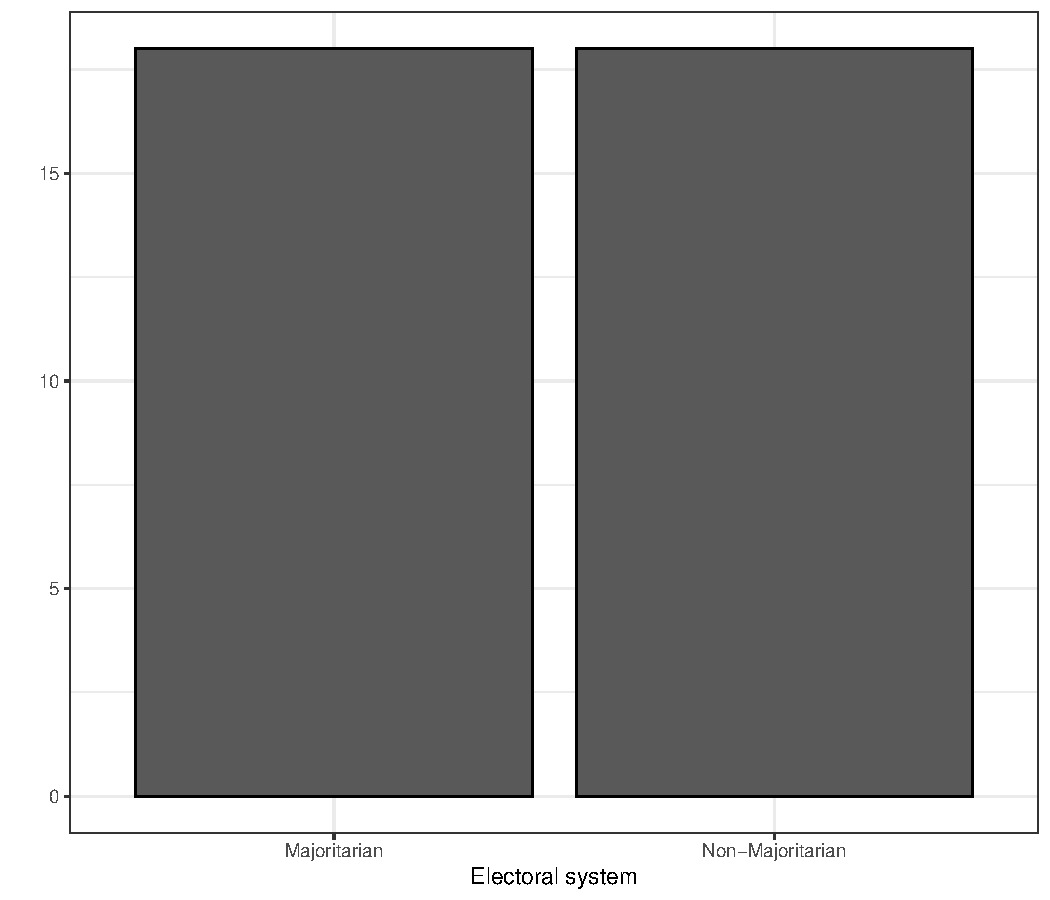
\includegraphics{appendixV5_files/figure-latex/unnamed-chunk-11-1.pdf}
\caption{Electoral system}
\end{figure}

\newpage

\hypertarget{electoral-system-x-sign-coefficient}{%
\subsubsection{Electoral system x Sign
Coefficient}\label{electoral-system-x-sign-coefficient}}

\begin{verbatim}
##           
##            Majoritarian Non-Majoritarian
##   Negative            5                8
##   Positive           13               10
\end{verbatim}

\begin{verbatim}
## 
##  Pearson's Chi-squared test with simulated p-value (based on 2000
##  replicates)
## 
## data:  table(dat$scoef, dat$elecsys2)
## X-squared = 1.0836, df = NA, p-value = 0.4883
\end{verbatim}

\newpage

\hypertarget{independent-variable-x-sign-coefficient}{%
\subsubsection{Independent Variable x Sign
Coefficient}\label{independent-variable-x-sign-coefficient}}

\begin{verbatim}
##           
##             K  N logN
##   Negative  1 11    1
##   Positive  8 10    5
\end{verbatim}

\begin{verbatim}
## 
##  Pearson's Chi-squared test with simulated p-value (based on 2000
##  replicates)
## 
## data:  table(dat$scoef, dat$indepvar2)
## X-squared = 5.8309, df = NA, p-value = 0.06397
\end{verbatim}

\newpage

\hypertarget{dependent-variables-x-independent-variables}{%
\subsubsection{Dependent variables x Independent
variables}\label{dependent-variables-x-independent-variables}}

\begin{verbatim}
##           
##            ExpPC PCTGDP logExpPC
##   Negative     6      4        3
##   Positive    12      7        4
\end{verbatim}

\begin{verbatim}
## 
##  Pearson's Chi-squared test with simulated p-value (based on 2000
##  replicates)
## 
## data:  table(dat$scoef, dat$depvar2)
## X-squared = 0.19858, df = NA, p-value = 1
\end{verbatim}

\newpage

\hypertarget{meta-analysis}{%
\subsection{Meta-analysis}\label{meta-analysis}}

We combined the three independent variables (N, logN, and K) with the
levels of the three dependent variables (ExpPC, logExpPC, PCTGDP). This
formed a 3x3 possibility for our analysis.

\hypertarget{exppc-x-n}{%
\subsubsection{ExpPC x N}\label{exppc-x-n}}

\begin{verbatim}
##                                 SMD             95%-CI %W(random)
## Crowley (2019)              -0.3510 [-1.8112;  1.1092]        5.3
## Lee and Park (2018)         -0.8510 [-3.5851;  1.8831]        2.1
## Lee (2016)                   0.0164 [-2.5570;  2.5898]        2.4
## Kessler (2014)               0.1740 [ 0.0074;  0.3406]       13.1
## Bjedov et al. (2014)        -0.0030 [-0.0226;  0.0166]       13.4
## Baskaran (2013)              0.9740 [-0.1212;  2.0692]        7.3
## Erler (2007)                 3.9300 [ 1.6172;  6.2428]        2.8
## Chen and Malhotra (2007)    -2.0400 [-4.6468;  0.5668]        2.3
## Fiorino and Ricciuti (2007)  0.2130 [ 0.1777;  0.2483]       13.4
## Primo (2006)                -0.8200 [-1.1924; -0.4476]       12.2
## Matsusaka (2005)            -0.9600 [-1.3128; -0.6072]       12.3
## Schaltegger and Feld (2009)  0.0010 [-0.0010;  0.0030]       13.4
## 
## Number of studies combined: k = 12
## 
##                          SMD            95%-CI     t p-value
## Random effects model -0.0699 [-0.6712; 0.5314] -0.26  0.8028
## Prediction interval          [-1.5540; 1.4142]              
## 
## Quantifying heterogeneity:
##  tau^2 = 0.3690 [0.1794; 4.7570]; tau = 0.6075 [0.4236; 2.1810];
##  I^2 = 94.7% [92.3%; 96.3%]; H = 4.34 [3.61; 5.21]
## 
## Test of heterogeneity:
##       Q d.f.  p-value
##  206.92   11 < 0.0001
## 
## Details on meta-analytical method:
## - Inverse variance method
## - Restricted maximum-likelihood estimator for tau^2
## - Q-profile method for confidence interval of tau^2 and tau
## - Hartung-Knapp adjustment for random effects model
\end{verbatim}

And the forest plot:

\begin{figure}
\centering
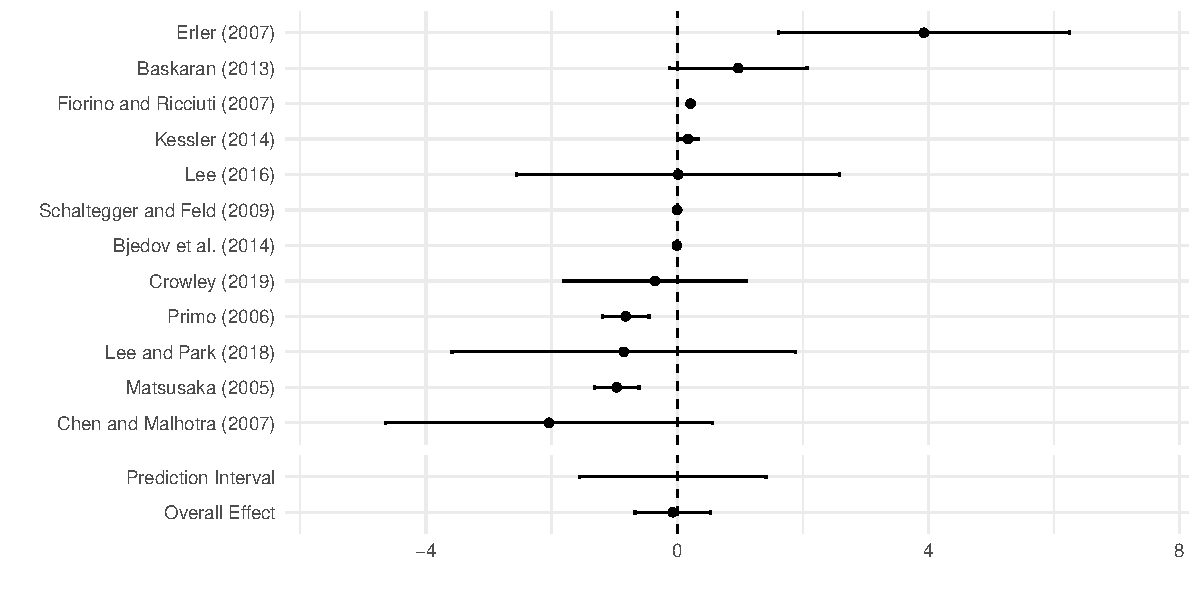
\includegraphics{appendixV5_files/figure-latex/unnamed-chunk-16-1.pdf}
\caption{Effect of lower houses size (N) on Per Capita Expenditure
(ExpPC)}
\end{figure}

Highlights:

\begin{enumerate}
\def\labelenumi{\arabic{enumi}.}
\tightlist
\item
  The results are highly heterogeneous: \$I\^{}2 = \$ 94.68.
\item
  The Random effects modem SMD estimated is \$g = \$ -0.07 (\(SE =\)
  0.273).
\item
  The prediction interval ranges from -1.55 to 1.41. Therefore, it
  emcompasses zero.
\end{enumerate}

\newpage

\hypertarget{electoral-system-subgroup-analysis}{%
\paragraph{Electoral system subgroup
analysis}\label{electoral-system-subgroup-analysis}}

The law of 1/n was created for majoritarian systems. In the theoretical
section below, we explain why the argument have potential issues when
applied to non-majoritarian electoral systems. We estimated a subgroup
analysis using a binary electoral system.

\begin{figure}
\centering
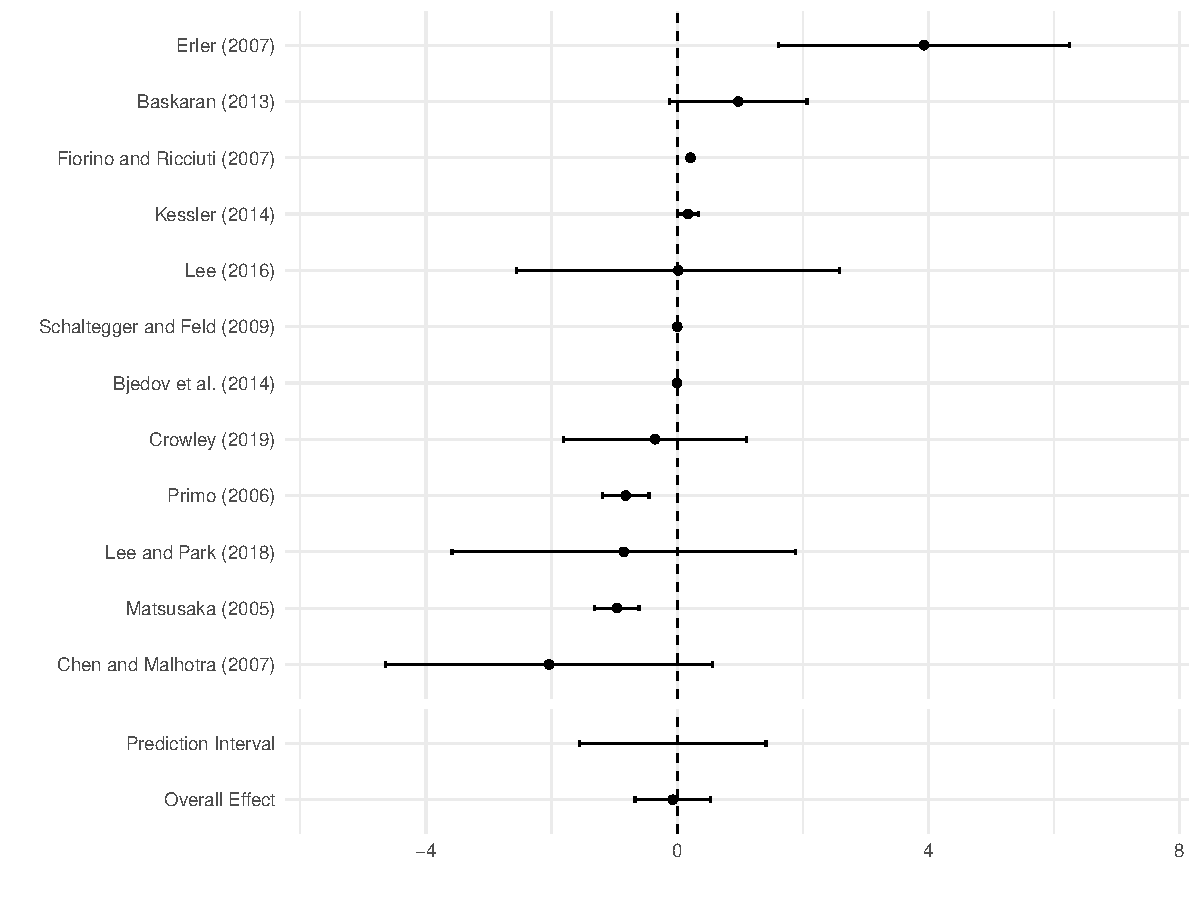
\includegraphics{appendixV5_files/figure-latex/unnamed-chunk-17-1.pdf}
\caption{Subgroup Analysis of (N) x (ExpPC), controlling by electoral
system}
\end{figure}

Therefore, we can see that the hypothesis that majoritarian systems
produce systematic positive effects was disproved. The majoritarian
systems in the sample had a random effects model estimate of -0.25,
while the random effects model in the non-majoritarian subgroup fitted a
value of 0.08. Both are non-significant, but they reassure us that the
absense of effect is not caused by pooling multiple types of electoral
systems.

\newpage

\hypertarget{pctgdp-x-n}{%
\subsubsection{PCTGDP x N}\label{pctgdp-x-n}}

This model fits the random effects for the percentage of GDP as public
expenditure as the main outcome, and the size of lower house as the main
treatment variable.

\begin{Shaded}
\begin{Highlighting}[]
\CommentTok{# Pooling effects analysis -- PCTGDP x N}
\NormalTok{aux <-}\StringTok{ }\NormalTok{dat }\OperatorTok
\StringTok{  }\KeywordTok{filter}\NormalTok{(indepvar2 }\OperatorTok{==}\StringTok{ 'N'}\NormalTok{,}
\NormalTok{         depvar2 }\OperatorTok{==}\StringTok{ 'PCTGDP'}\NormalTok{)}

\NormalTok{mod <-}\StringTok{ }\KeywordTok{metagen}\NormalTok{(coef, SE, }\DataTypeTok{data=}\NormalTok{aux, }
          \DataTypeTok{studlab=}\KeywordTok{paste}\NormalTok{(authoryear),}
          \DataTypeTok{comb.fixed =} \OtherTok{FALSE}\NormalTok{,}
          \DataTypeTok{comb.random =} \OtherTok{TRUE}\NormalTok{,}
          \DataTypeTok{method.tau =} \StringTok{"REML"}\NormalTok{,}
          \DataTypeTok{hakn =} \OtherTok{TRUE}\NormalTok{,}
          \DataTypeTok{prediction=}\OtherTok{TRUE}\NormalTok{,}
          \DataTypeTok{sm=}\StringTok{"SMD"}\NormalTok{)}
\NormalTok{mod}
\end{Highlighting}
\end{Shaded}

\begin{verbatim}
##                               SMD             95%-CI %W(random)
## Bjedov et al. (2014)      -0.0040 [-0.0432;  0.0352]       15.1
## Maldonado (2013)          -0.0609 [-0.0838; -0.0380]       19.5
## Mukherjee (2003)           0.0030 [ 0.0010;  0.0050]       23.0
## Bradbury and Crain (2001)  0.0036 [ 0.0008;  0.0065]       23.0
## Ricciuti (2004)            0.0140 [-0.0095;  0.0375]       19.4
## 
## Number of studies combined: k = 5
## 
##                          SMD            95%-CI     t p-value
## Random effects model -0.0083 [-0.0450; 0.0285] -0.62  0.5667
## Prediction interval          [-0.1054; 0.0889]              
## 
## Quantifying heterogeneity:
##  tau^2 = 0.0008 [0.0002; 0.0072]; tau = 0.0275 [0.0129; 0.0849];
##  I^2 = 87.1% [72.2%; 94.0%]; H = 2.78 [1.90; 4.08]
## 
## Test of heterogeneity:
##      Q d.f.  p-value
##  30.97    4 < 0.0001
## 
## Details on meta-analytical method:
## - Inverse variance method
## - Restricted maximum-likelihood estimator for tau^2
## - Q-profile method for confidence interval of tau^2 and tau
## - Hartung-Knapp adjustment for random effects model
\end{verbatim}

And the forest plot:

\begin{figure}
\centering
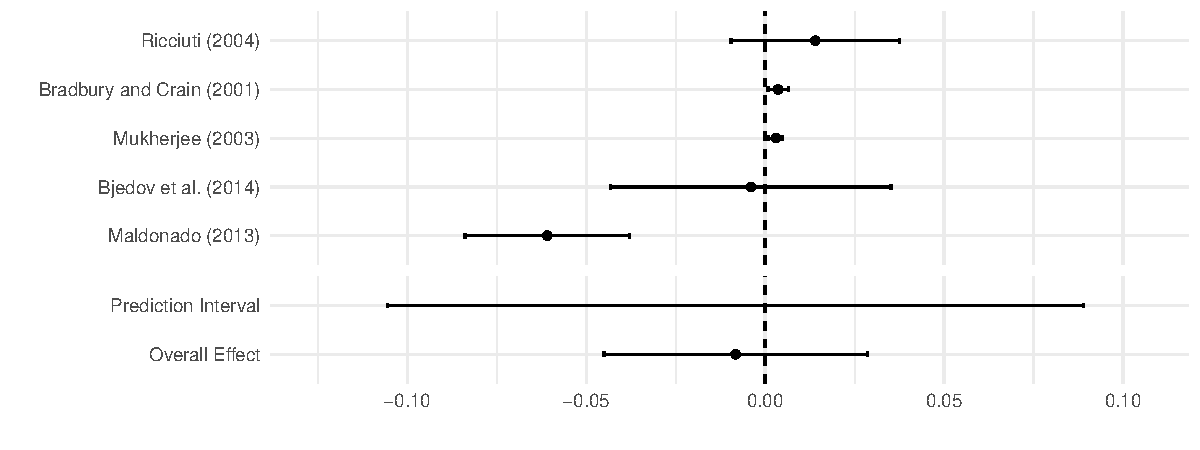
\includegraphics{appendixV5_files/figure-latex/unnamed-chunk-19-1.pdf}
\caption{Effect of lower houses size (N) on percentage of public
expenditure GDP (PCTGDP)}
\end{figure}

Highlights:

\begin{enumerate}
\def\labelenumi{\arabic{enumi}.}
\tightlist
\item
  The results are highly heterogeneous: \$I\^{}2 = \$ 87.08.
\item
  The Random effects modem SMD estimated is \$g = \$ -0.01 (\(SE =\)
  0.013).
\item
  The prediction interval ranges from -0.11 to 0.09. Therefore, it
  emcompasses zero.
\end{enumerate}

\newpage

\hypertarget{logexppc-x-n}{%
\subsubsection{logExpPC x N}\label{logexppc-x-n}}

This model estimates the Log of Per Capita Expenditure as the dependent
variable, and the number of lower house legislators as the treatment
variable.

\begin{Shaded}
\begin{Highlighting}[]
\CommentTok{# Pooling effects analysis -- logExpPC x N}
\NormalTok{aux <-}\StringTok{ }\NormalTok{dat }\OperatorTok
\StringTok{  }\KeywordTok{filter}\NormalTok{(indepvar2 }\OperatorTok{==}\StringTok{ 'N'}\NormalTok{,}
\NormalTok{         depvar2 }\OperatorTok{==}\StringTok{ 'logExpPC'}\NormalTok{)}

\NormalTok{mod <-}\StringTok{ }\KeywordTok{metagen}\NormalTok{(}
\NormalTok{  coef, SE, }\DataTypeTok{data=}\NormalTok{aux, }
  \DataTypeTok{studlab=}\KeywordTok{paste}\NormalTok{(authoryear),}
  \DataTypeTok{comb.fixed =} \OtherTok{FALSE}\NormalTok{,}
  \DataTypeTok{comb.random =} \OtherTok{TRUE}\NormalTok{,}
  \DataTypeTok{method.tau =} \StringTok{"REML"}\NormalTok{,}
  \DataTypeTok{hakn =} \OtherTok{TRUE}\NormalTok{,}
  \DataTypeTok{prediction =} \OtherTok{TRUE}\NormalTok{,}
  \DataTypeTok{sm=}\StringTok{"SMD"}
\NormalTok{  )}

\NormalTok{mod}
\end{Highlighting}
\end{Shaded}

\begin{verbatim}
##                              SMD             95%-CI %W(random)
## Lewis (2019)             -0.1740 [-0.2450; -0.1030]       24.3
## Höhmann (2017)           -0.0300 [-0.0496; -0.0104]       26.6
## Drew and Dollery (2017)   0.0770 [ 0.0221;  0.1319]       25.3
## Pettersson-Lidbom (2012) -0.1590 [-0.2394; -0.0786]       23.7
## 
## Number of studies combined: k = 4
## 
##                          SMD            95%-CI     t p-value
## Random effects model -0.0686 [-0.2560; 0.1188] -1.17  0.3282
## Prediction interval          [-0.6179; 0.4807]              
## 
## Quantifying heterogeneity:
##  tau^2 = 0.0128 [0.0034; 0.1933]; tau = 0.1133 [0.0584; 0.4396];
##  I^2 = 92.5% [84.1%; 96.5%]; H = 3.66 [2.51; 5.34]
## 
## Test of heterogeneity:
##      Q d.f.  p-value
##  40.11    3 < 0.0001
## 
## Details on meta-analytical method:
## - Inverse variance method
## - Restricted maximum-likelihood estimator for tau^2
## - Q-profile method for confidence interval of tau^2 and tau
## - Hartung-Knapp adjustment for random effects model
\end{verbatim}

And the forest plot:

\begin{figure}
\centering
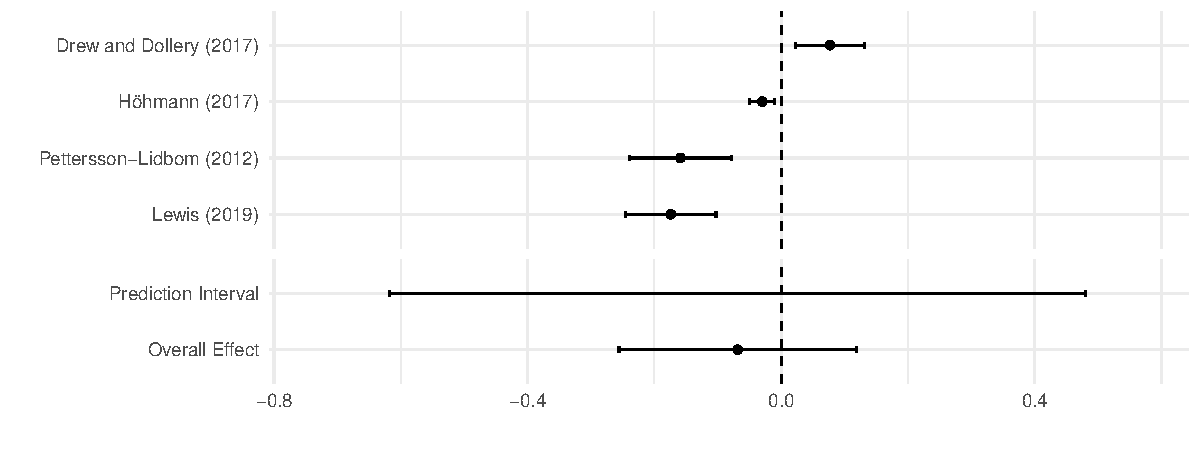
\includegraphics{appendixV5_files/figure-latex/unnamed-chunk-21-1.pdf}
\caption{Effect of lower houses size (N) on log of per capita
expenditure (logExpPC)}
\end{figure}

Highlights:

\begin{enumerate}
\def\labelenumi{\arabic{enumi}.}
\tightlist
\item
  The results are highly heterogeneous: \$I\^{}2 = \$ 92.52.
\item
  The Random effects modem SMD estimated is \$g = \$ -0.07 (\(SE =\)
  0.059).
\item
  The prediction interval ranges from -0.62 to 0.48. Therefore, it
  emcompasses zero.
\end{enumerate}

\newpage

\hypertarget{exppc-x-logn}{%
\subsubsection{ExpPC x logN}\label{exppc-x-logn}}

There were no studies that had per capita expenditure in the dependent
variable and log of lower house size in the treatment variable.

\hypertarget{pctgdp-x-logn}{%
\subsubsection{PCTGDP x logN}\label{pctgdp-x-logn}}

This meta-regression investigates the percentage of GDP as public
expenditure as the dependent variable and the log lower house size
(logN) as the treatment variable.

\begin{Shaded}
\begin{Highlighting}[]
\CommentTok{# Pooling effects analysis -- PCTGDP x logN}
\NormalTok{aux <-}\StringTok{ }\NormalTok{dat }\OperatorTok
\StringTok{  }\KeywordTok{filter}\NormalTok{(indepvar2 }\OperatorTok{==}\StringTok{ 'logN'}\NormalTok{,}
\NormalTok{         depvar2 }\OperatorTok{==}\StringTok{ 'PCTGDP'}\NormalTok{)}

\NormalTok{mod <-}\StringTok{ }\KeywordTok{metagen}\NormalTok{(}
\NormalTok{  coef, SE, }\DataTypeTok{data=}\NormalTok{aux, }
  \DataTypeTok{studlab=}\KeywordTok{paste}\NormalTok{(authoryear),}
  \DataTypeTok{comb.fixed =} \OtherTok{FALSE}\NormalTok{,}
  \DataTypeTok{comb.random =} \OtherTok{TRUE}\NormalTok{,}
  \DataTypeTok{method.tau =} \StringTok{"REML"}\NormalTok{,}
  \DataTypeTok{hakn =} \OtherTok{TRUE}\NormalTok{,}
  \DataTypeTok{prediction=}\OtherTok{TRUE}\NormalTok{,}
  \DataTypeTok{sm=}\StringTok{"SMD"}
\NormalTok{  )}

\NormalTok{mod}
\end{Highlighting}
\end{Shaded}

\begin{verbatim}
##                         SMD            95%-CI %W(random)
## Baqir (1999)         2.0660 [ 1.4887; 2.6433]       40.8
## Lledo (2003)        -4.6900 [-9.9427; 0.5627]       17.7
## Stein et al. (1998)  0.0109 [-0.0171; 0.0389]       41.5
## 
## Number of studies combined: k = 3
## 
##                         SMD              95%-CI    t p-value
## Random effects model 0.0203 [ -7.1961;  7.2367] 0.01  0.9914
## Prediction interval         [-36.2058; 36.2465]             
## 
## Quantifying heterogeneity:
##  tau^2 = 5.3156 [0.5756; >100.0000]; tau = 2.3056 [0.7587; >10.0000];
##  I^2 = 96.1% [91.8%; 98.2%]; H = 5.08 [3.48; 7.42]
## 
## Test of heterogeneity:
##      Q d.f.  p-value
##  51.65    2 < 0.0001
## 
## Details on meta-analytical method:
## - Inverse variance method
## - Restricted maximum-likelihood estimator for tau^2
## - Q-profile method for confidence interval of tau^2 and tau
## - Hartung-Knapp adjustment for random effects model
\end{verbatim}

And the forest plot:

\begin{figure}
\centering
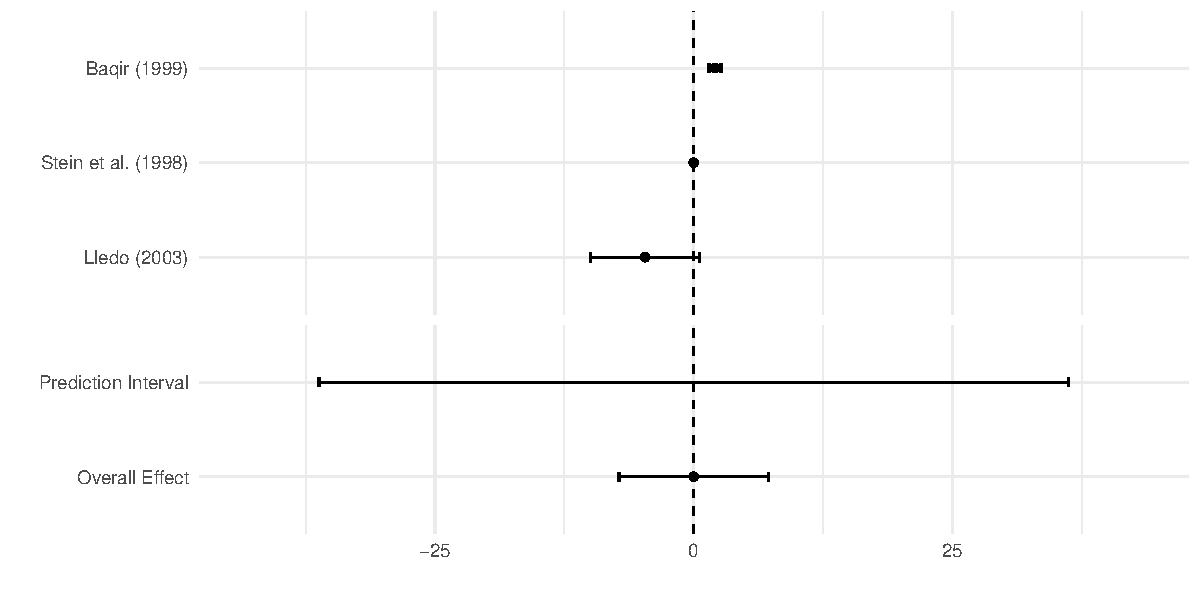
\includegraphics{appendixV5_files/figure-latex/unnamed-chunk-23-1.pdf}
\caption{Effect of log lower houses size (logN) on the GDP share of
public expenditure (PCTGDP)}
\end{figure}

Highlights:

\begin{enumerate}
\def\labelenumi{\arabic{enumi}.}
\tightlist
\item
  The results are highly heterogeneous: \$I\^{}2 = \$ 96.13.
\item
  The Random effects modem SMD estimated is \$g = \$ 0.02 (\(SE =\)
  1.677).
\item
  The prediction interval ranges from -36.21 to 36.25. Therefore, it
  emcompasses zero.
\end{enumerate}

\newpage

\hypertarget{logexppc-x-logn}{%
\subsubsection{logExpPC x logN}\label{logexppc-x-logn}}

In this specification, we study the log of per capita expenditure
(logExpPC) as a function of the log of lower house size (logN).

\begin{Shaded}
\begin{Highlighting}[]
\CommentTok{# Pooling effects analysis -- logExpPC x logN}
\NormalTok{aux <-}\StringTok{ }\NormalTok{dat }\OperatorTok
\StringTok{  }\KeywordTok{filter}\NormalTok{(indepvar2 }\OperatorTok{==}\StringTok{ 'logN'}\NormalTok{,}
\NormalTok{         depvar2 }\OperatorTok{==}\StringTok{ 'logExpPC'}\NormalTok{)}

\NormalTok{mod <-}\StringTok{ }\KeywordTok{metagen}\NormalTok{(coef, SE, }\DataTypeTok{data=}\NormalTok{aux, }
          \DataTypeTok{studlab=}\KeywordTok{paste}\NormalTok{(authoryear),}
          \DataTypeTok{comb.fixed =} \OtherTok{FALSE}\NormalTok{,}
          \DataTypeTok{comb.random =} \OtherTok{TRUE}\NormalTok{,}
          \DataTypeTok{method.tau =} \StringTok{"REML"}\NormalTok{,}
          \DataTypeTok{hakn =} \OtherTok{TRUE}\NormalTok{,}
          \DataTypeTok{prediction=}\OtherTok{TRUE}\NormalTok{,}
          \DataTypeTok{sm=}\StringTok{"SMD"}\NormalTok{)}
\NormalTok{mod}
\end{Highlighting}
\end{Shaded}

\begin{verbatim}
##                     SMD           95%-CI %W(random)
## MacDonald (2008) 0.1360 [0.0447; 0.2273]       31.9
## Baqir (2002)     0.1127 [0.0396; 0.1858]       34.2
## Baqir (1999)     0.3020 [0.2269; 0.3771]       33.9
## 
## Number of studies combined: k = 3
## 
##                         SMD            95%-CI    t p-value
## Random effects model 0.1844 [-0.0738; 0.4425] 3.07  0.0916
## Prediction interval         [-1.2580; 1.6267]             
## 
## Quantifying heterogeneity:
##  tau^2 = 0.0093 [0.0014; 0.4193]; tau = 0.0964 [0.0372; 0.6476];
##  I^2 = 85.9% [59.0%; 95.2%]; H = 2.66 [1.56; 4.54]
## 
## Test of heterogeneity:
##      Q d.f. p-value
##  14.18    2  0.0008
## 
## Details on meta-analytical method:
## - Inverse variance method
## - Restricted maximum-likelihood estimator for tau^2
## - Q-profile method for confidence interval of tau^2 and tau
## - Hartung-Knapp adjustment for random effects model
\end{verbatim}

And the forest plot:

\begin{figure}
\centering
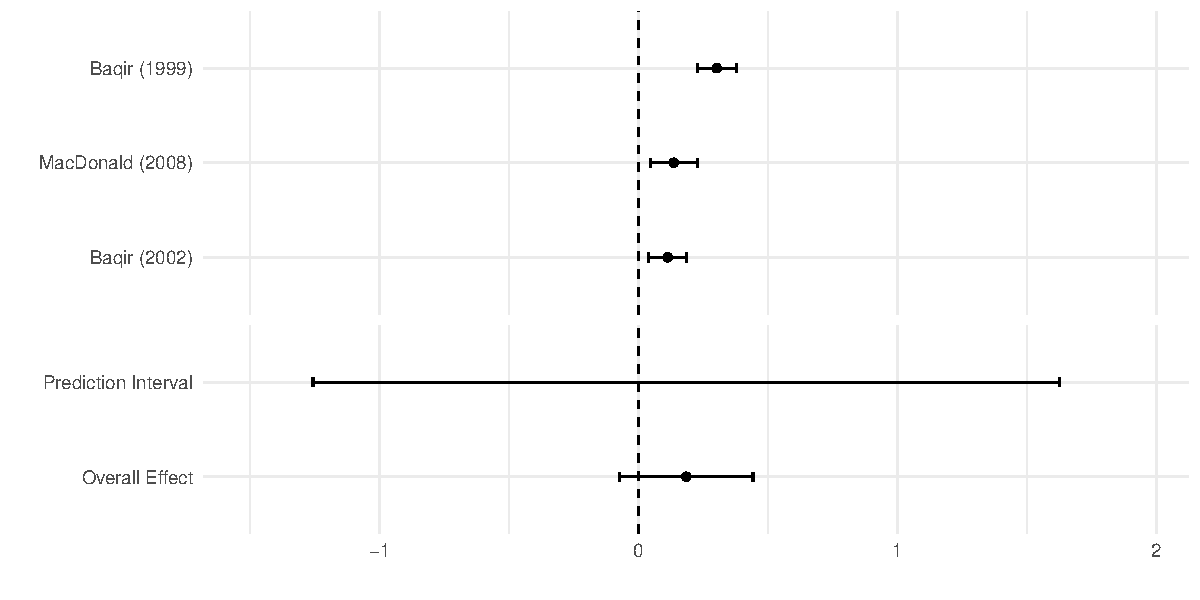
\includegraphics{appendixV5_files/figure-latex/unnamed-chunk-25-1.pdf}
\caption{Effect of log lower houses size (logN) on the log of per capita
government expenditure (logExpPC)}
\end{figure}

Highlights:

\begin{enumerate}
\def\labelenumi{\arabic{enumi}.}
\tightlist
\item
  The results are highly heterogeneous: \$I\^{}2 = \$ 85.9.
\item
  The Random effects modem SMD estimated is \$g = \$ 0.18 (\(SE =\)
  0.06). \textbf{This model is significant at the 10\% confidence
  level.}
\item
  The prediction interval ranges from -1.26 to 1.63. Therefore, it
  emcompasses zero.
\end{enumerate}

\newpage

\hypertarget{exppc-x-k}{%
\subsubsection{ExpPC x K}\label{exppc-x-k}}

Now we are investigating the upper house size (K). In this model, we
investigate the effect of upper house size on expenditure per capita
(ExpPC).

\begin{Shaded}
\begin{Highlighting}[]
\CommentTok{# Pooling effects analysis -- ExpPC x K}
\NormalTok{aux <-}\StringTok{ }\NormalTok{dat }\OperatorTok
\StringTok{  }\KeywordTok{filter}\NormalTok{(indepvar2 }\OperatorTok{==}\StringTok{ 'K'}\NormalTok{,}
\NormalTok{         depvar2 }\OperatorTok{==}\StringTok{ 'ExpPC'}\NormalTok{)}

\NormalTok{mod <-}\StringTok{ }\KeywordTok{metagen}\NormalTok{(coef, SE, }\DataTypeTok{data=}\NormalTok{aux, }
          \DataTypeTok{studlab=}\KeywordTok{paste}\NormalTok{(authoryear),}
          \DataTypeTok{comb.fixed =} \OtherTok{FALSE}\NormalTok{,}
          \DataTypeTok{comb.random =} \OtherTok{TRUE}\NormalTok{,}
          \DataTypeTok{method.tau =} \StringTok{"REML"}\NormalTok{,}
          \DataTypeTok{hakn =} \OtherTok{TRUE}\NormalTok{,}
          \DataTypeTok{prediction=}\OtherTok{TRUE}\NormalTok{,}
          \DataTypeTok{sm=}\StringTok{"SMD"}\NormalTok{)}
\NormalTok{mod}
\end{Highlighting}
\end{Shaded}

\begin{verbatim}
##                                    SMD             95%-CI %W(random)
## Crowley (2019)                  8.2100 [ 0.2702; 16.1498]       20.0
## Lee and Park (2018)            19.7400 [ 3.2645; 36.2155]       13.8
## Lee (2016)                     38.4400 [ 0.7499; 76.1301]        5.1
## Bradbury and Stephenson (2009)  0.6240 [ 0.2295;  1.0185]       23.1
## Chen and Malhotra (2007)       26.0900 [11.4883; 40.6917]       15.1
## Primo (2006)                    0.9700 [-0.4804;  2.4204]       23.0
## 
## Number of studies combined: k = 6
## 
##                          SMD              95%-CI    t p-value
## Random effects model 10.6134 [ -2.6210; 23.8479] 2.06  0.0943
## Prediction interval          [-21.1303; 42.3571]             
## 
## Quantifying heterogeneity:
##  tau^2 = 104.2124 [20.3551; >1042.1236]; tau = 10.2084 [4.5117; >32.2819];
##  I^2 = 79.4% [55.1%; 90.6%]; H = 2.20 [1.49; 3.26]
## 
## Test of heterogeneity:
##      Q d.f. p-value
##  24.31    5  0.0002
## 
## Details on meta-analytical method:
## - Inverse variance method
## - Restricted maximum-likelihood estimator for tau^2
## - Q-profile method for confidence interval of tau^2 and tau
## - Hartung-Knapp adjustment for random effects model
\end{verbatim}

And the forest plot:

\begin{figure}
\centering
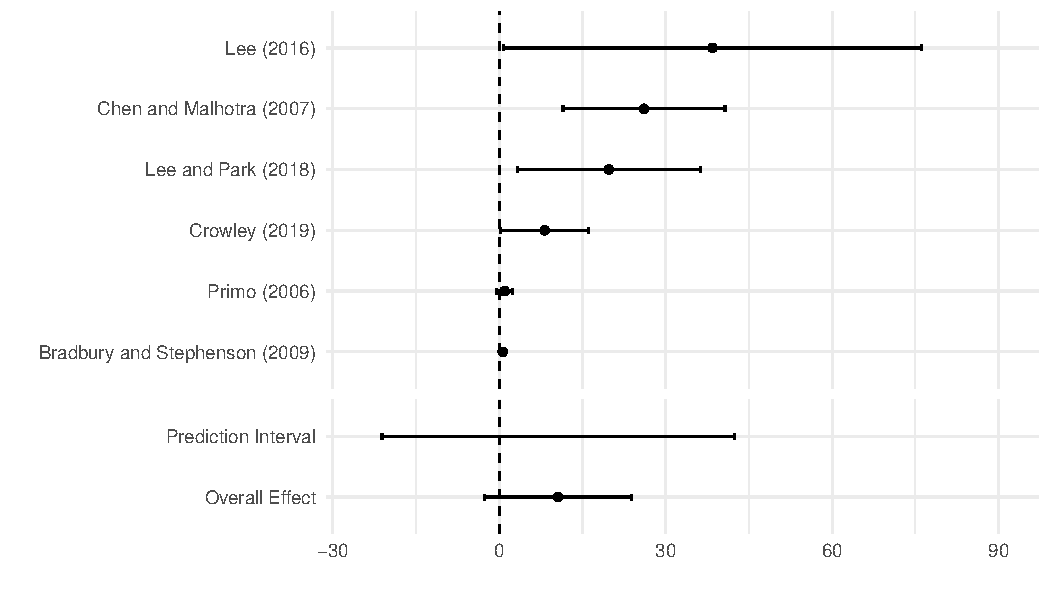
\includegraphics{appendixV5_files/figure-latex/unnamed-chunk-27-1.pdf}
\caption{Effect of upper house size (K) on the per capita government
expenditure (ExpPC)}
\end{figure}

Highlights:

\begin{enumerate}
\def\labelenumi{\arabic{enumi}.}
\tightlist
\item
  The results are highly heterogeneous: \$I\^{}2 = \$ 79.43.
\item
  The Random effects modem SMD estimated is \$g = \$ 10.61 (\(SE =\)
  5.148).
\item
  The prediction interval ranges from -21.13 to 42.36. Therefore, it
  emcompasses zero.
\end{enumerate}

\newpage

\hypertarget{pctgdp-x-k}{%
\subsubsection{PCTGDP x K}\label{pctgdp-x-k}}

This model looks into the effect of upper house size (K) on the public
expenditure share of the GDP (PCTGDP).

\begin{Shaded}
\begin{Highlighting}[]
\CommentTok{# Pooling effects analysis -- PCTGDP x K}
\NormalTok{aux <-}\StringTok{ }\NormalTok{dat }\OperatorTok
\StringTok{  }\KeywordTok{filter}\NormalTok{(indepvar2 }\OperatorTok{==}\StringTok{ 'K'}\NormalTok{,}
\NormalTok{         depvar2 }\OperatorTok{==}\StringTok{ 'PCTGDP'}\NormalTok{)}

\NormalTok{mod <-}\StringTok{ }\KeywordTok{metagen}\NormalTok{(coef, SE, }\DataTypeTok{data=}\NormalTok{aux, }
          \DataTypeTok{studlab=}\KeywordTok{paste}\NormalTok{(authoryear),}
          \DataTypeTok{comb.fixed =} \OtherTok{FALSE}\NormalTok{,}
          \DataTypeTok{comb.random =} \OtherTok{TRUE}\NormalTok{,}
          \DataTypeTok{method.tau =} \StringTok{"REML"}\NormalTok{,}
          \DataTypeTok{hakn =} \OtherTok{TRUE}\NormalTok{,}
          \DataTypeTok{prediction=}\OtherTok{TRUE}\NormalTok{,}
          \DataTypeTok{sm=}\StringTok{"SMD"}\NormalTok{)}
\NormalTok{mod}
\end{Highlighting}
\end{Shaded}

\begin{verbatim}
##                               SMD             95%-CI %W(random)
## Maldonado (2012)          -0.0400 [-0.0659; -0.0141]       31.3
## Bradbury and Crain (2001)  0.0126 [ 0.0010;  0.0243]       36.4
## Ricciuti (2004)            0.0160 [-0.0075;  0.0395]       32.3
## 
## Number of studies combined: k = 3
## 
##                          SMD            95%-CI     t p-value
## Random effects model -0.0027 [-0.0793; 0.0738] -0.15  0.8915
## Prediction interval          [-0.4284; 0.4229]              
## 
## Quantifying heterogeneity:
##  tau^2 = 0.0008 [0.0001; 0.0388]; tau = 0.0284 [0.0101; 0.1970];
##  I^2 = 85.8% [58.6%; 95.1%]; H = 2.65 [1.55; 4.53]
## 
## Test of heterogeneity:
##      Q d.f. p-value
##  14.07    2  0.0009
## 
## Details on meta-analytical method:
## - Inverse variance method
## - Restricted maximum-likelihood estimator for tau^2
## - Q-profile method for confidence interval of tau^2 and tau
## - Hartung-Knapp adjustment for random effects model
\end{verbatim}

And the forest plot:

\begin{figure}
\centering
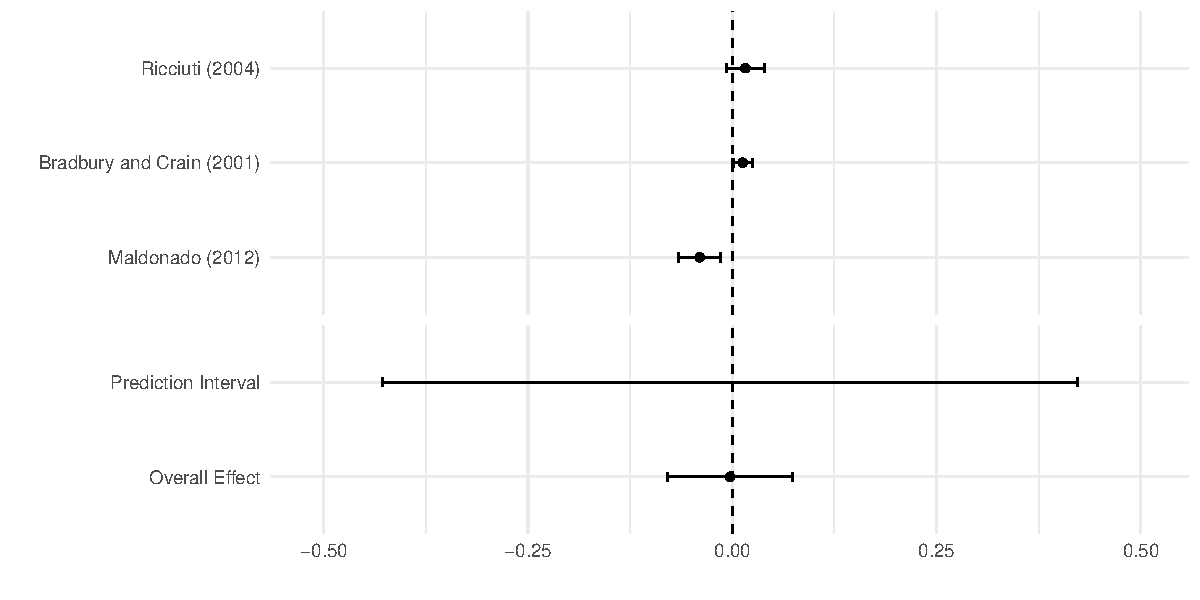
\includegraphics{appendixV5_files/figure-latex/unnamed-chunk-29-1.pdf}
\caption{Effect of upper house size (K) on the public expenditure share
of the GDP (PCTGDP)}
\end{figure}

Highlights:

\begin{enumerate}
\def\labelenumi{\arabic{enumi}.}
\tightlist
\item
  The results are highly heterogeneous: \$I\^{}2 = \$ 85.79.
\item
  The Random effects modem SMD estimated is \$g = \$ 0 (\(SE =\) 0.018).
\item
  The prediction interval ranges from -0.43 to 0.42. Therefore, it
  emcompasses zero.
\end{enumerate}

\newpage

\hypertarget{logexppc-x-k}{%
\subsubsection{logExpPC x K}\label{logexppc-x-k}}

No studies related the log of per capita expenditure with the size of
upper house (K).


\includegraphics{appendixV5_files/figure-latex/unnamed-chunk-30-2.pdf}
%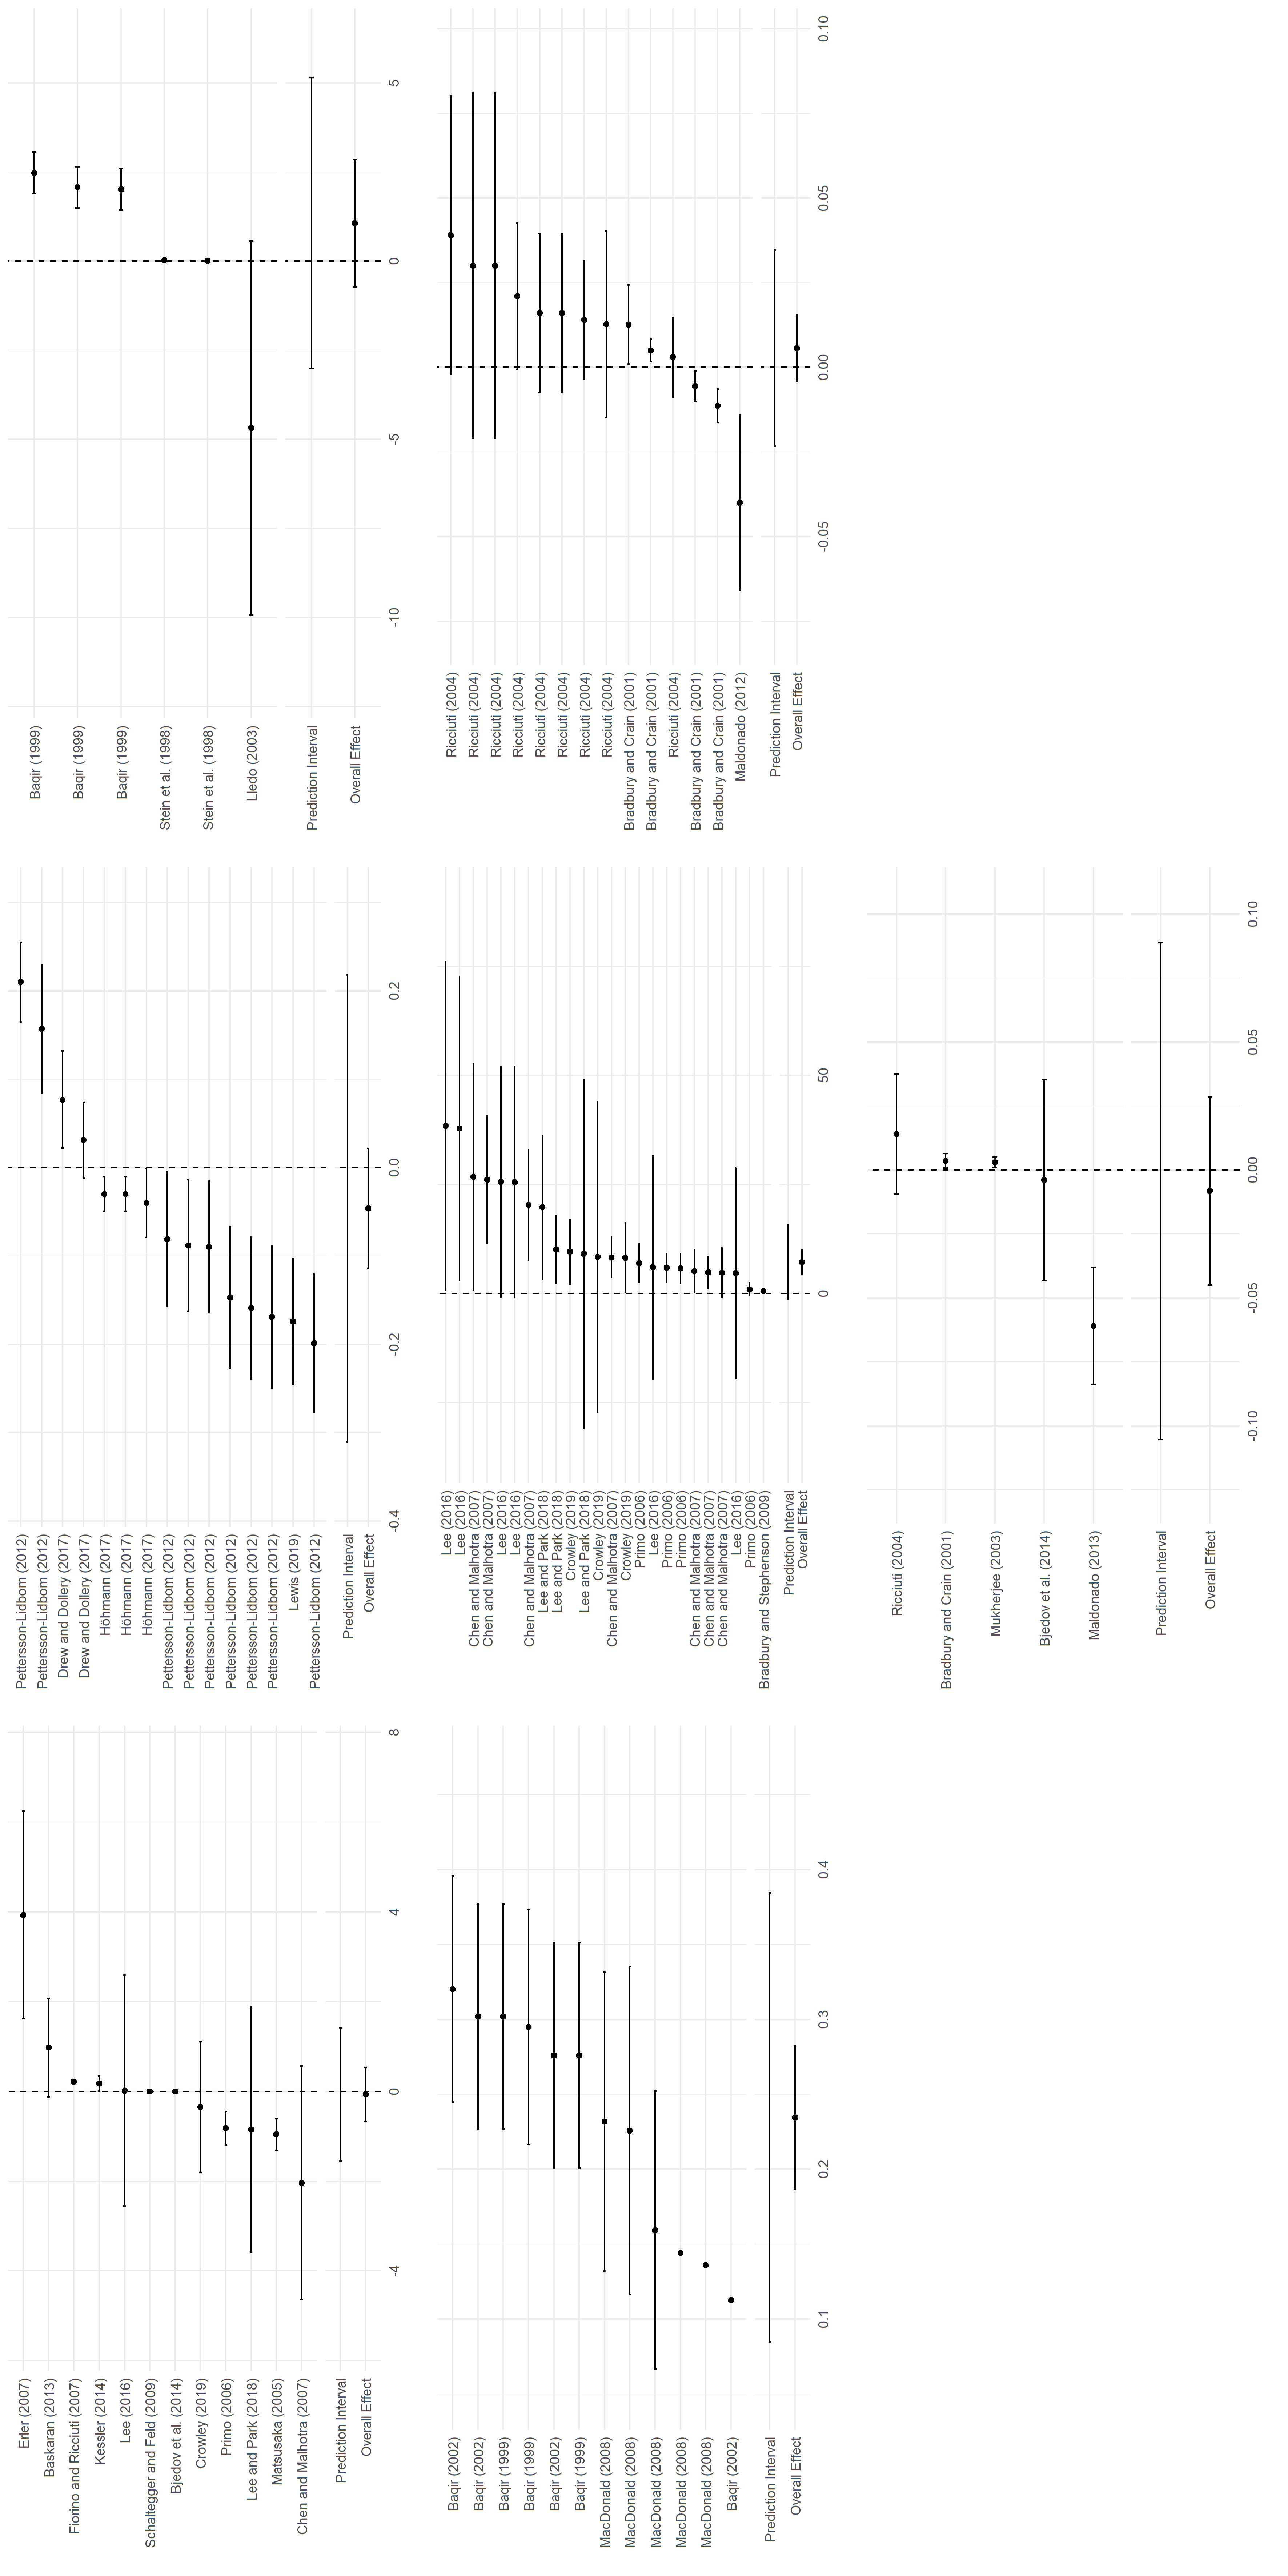
\includegraphics[width=49.21in]{appendixV5_files/figure-latex/unnamed-chunk-30-1}

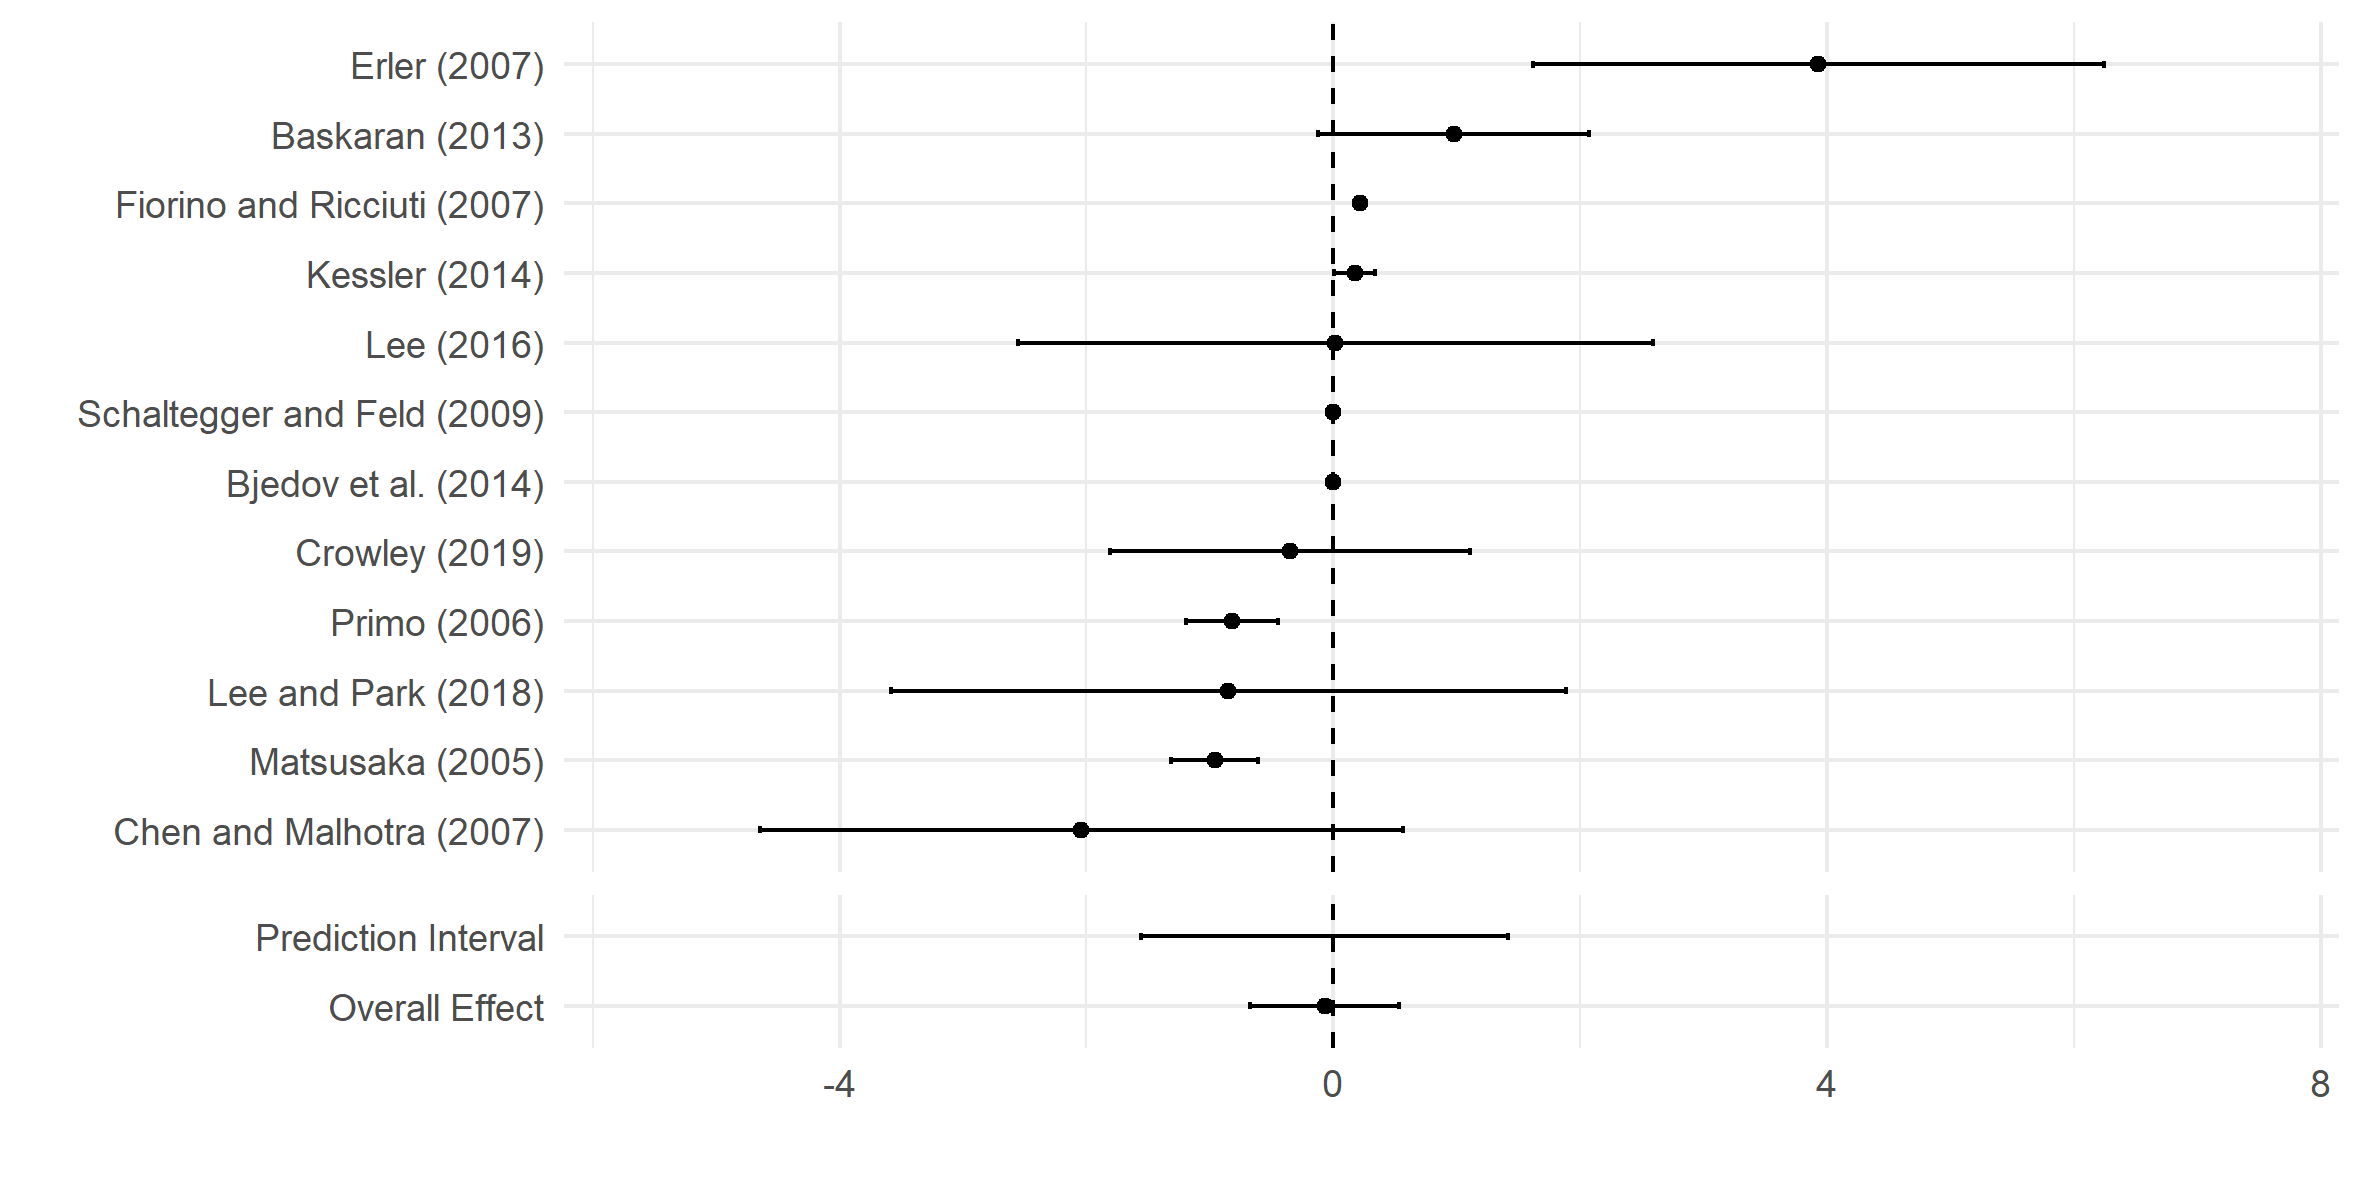
\includegraphics[width=20.21in]{plots/f1.png}


\newpage

\hypertarget{meta-analysis-all-coefficients}{%
\subsection{Meta-Analysis (all
coefficients)}\label{meta-analysis-all-coefficients}}

\hypertarget{exppc-x-n-1}{%
\subsubsection{ExpPC x N}\label{exppc-x-n-1}}

\begin{verbatim}
## Warning in rma.uni(yi = TE[sel], sei = seTE[sel], method = method.tau, control
## = control): Ratio of largest to smallest sampling variance extremely large. May
## not be able to obtain stable results.
\end{verbatim}

\begin{verbatim}
##                                 SMD             95%-CI %W(random)
## Crowley (2019)              -0.3510 [-1.8112;  1.1092]        2.0
## Crowley (2019)               5.9750 [ 0.7889; 11.1611]        0.3
## Crowley (2019)               7.6580 [-0.0290; 15.3450]        0.2
## Lee and Park (2018)         -0.8510 [-3.5851;  1.8831]        0.9
## Lee and Park (2018)         -1.6890 [-3.0551; -0.3229]        2.1
## Lee and Park (2018)          7.6320 [ 3.1064; 12.1576]        0.4
## Lee (2016)                   0.0164 [-2.5570;  2.5898]        1.0
## Kessler (2014)               0.1740 [ 0.0074;  0.3406]        3.6
## Kessler (2014)               0.2230 [ 0.1211;  0.3249]        3.6
## Kessler (2014)               0.2150 [ 0.0954;  0.3346]        3.6
## Kessler (2014)               0.1580 [ 0.0522;  0.2638]        3.6
## Bjedov et al. (2014)        -0.0030 [-0.0226;  0.0166]        3.6
## Bjedov et al. (2014)        -0.0060 [-0.0256;  0.0136]        3.6
## Baskaran (2013)              0.9740 [-0.1212;  2.0692]        2.5
## Erler (2007)                 3.9300 [ 1.6172;  6.2428]        1.2
## Chen and Malhotra (2007)    -2.0400 [-4.6468;  0.5668]        1.0
## Chen and Malhotra (2007)    -1.4000 [-2.6544; -0.1456]        2.3
## Fiorino and Ricciuti (2007)  0.2130 [ 0.1777;  0.2483]        3.6
## Fiorino and Ricciuti (2007)  0.2290 [ 0.1565;  0.3015]        3.6
## Fiorino and Ricciuti (2007)  0.4550 [ 0.3805;  0.5295]        3.6
## Fiorino and Ricciuti (2007)  0.4110 [ 0.3150;  0.5070]        3.6
## Fiorino and Ricciuti (2007)  0.2260 [ 0.1221;  0.3299]        3.6
## Fiorino and Ricciuti (2007)  0.2130 [-0.4083;  0.8343]        3.1
## Fiorino and Ricciuti (2007)  0.1850 [-0.4128;  0.7828]        3.2
## Fiorino and Ricciuti (2007)  0.2350 [-0.4235;  0.8935]        3.1
## Fiorino and Ricciuti (2007)  0.3740 [ 0.2486;  0.4994]        3.6
## Fiorino and Ricciuti (2007)  0.8110 [ 0.4562;  1.1658]        3.4
## Fiorino and Ricciuti (2007)  0.7950 [ 0.4500;  1.1400]        3.5
## Fiorino and Ricciuti (2007)  0.8490 [ 0.3825;  1.3155]        3.3
## Primo (2006)                -0.8200 [-1.1924; -0.4476]        3.4
## Primo (2006)                -1.7000 [-2.3076; -1.0924]        3.2
## Primo (2006)                -2.3700 [-3.0952; -1.6448]        3.0
## Primo (2006)                -2.0300 [-2.7552; -1.3048]        3.0
## Matsusaka (2005)            -0.9600 [-1.3128; -0.6072]        3.4
## Schaltegger and Feld (2009)  0.0010 [-0.0010;  0.0030]        3.6
## Schaltegger and Feld (2009) -0.0010 [-0.0030;  0.0010]        3.6
## 
## Number of studies combined: k = 36
## 
##                          SMD            95%-CI     t p-value
## Random effects model -0.0169 [-0.4166; 0.3829] -0.09  0.9322
## Prediction interval          [-1.7588; 1.7250]              
## 
## Quantifying heterogeneity:
##  tau^2 = 0.6959 [0.7202; 4.3553]; tau = 0.8342 [0.8486; 2.0869];
##  I^2 = 95.3% [94.2%; 96.1%]; H = 4.60 [4.16; 5.08]
## 
## Test of heterogeneity:
##       Q d.f.  p-value
##  739.53   35 < 0.0001
## 
## Details on meta-analytical method:
## - Inverse variance method
## - Restricted maximum-likelihood estimator for tau^2
## - Q-profile method for confidence interval of tau^2 and tau
## - Hartung-Knapp adjustment for random effects model
\end{verbatim}

And the forest plot:

\begin{figure}
\centering
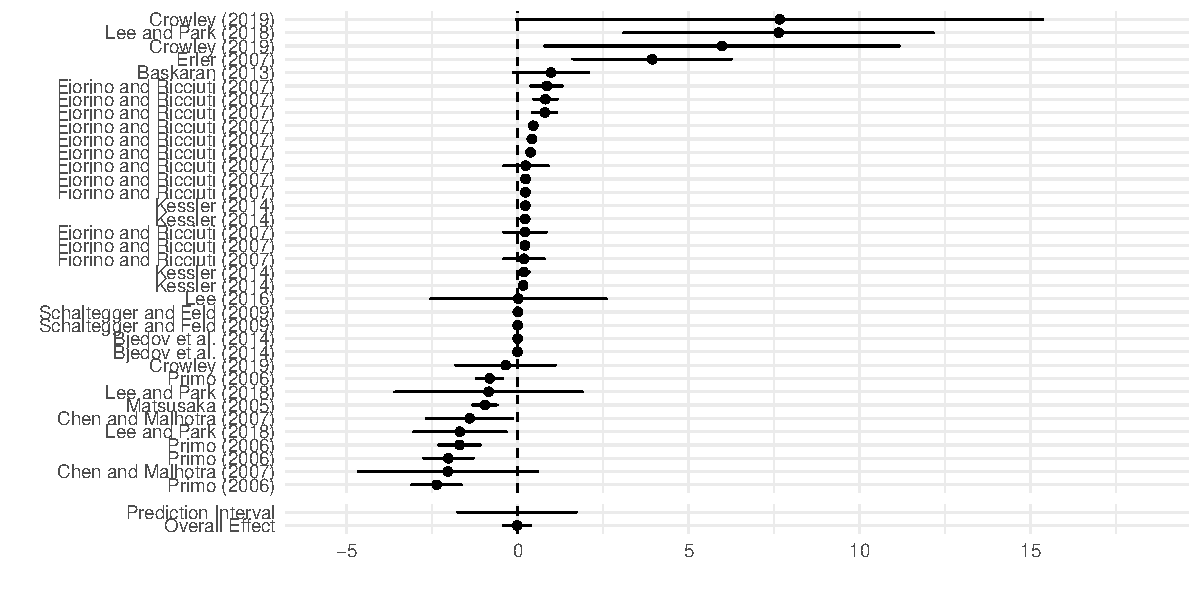
\includegraphics{appendixV5_files/figure-latex/unnamed-chunk-32-1.pdf}
\caption{Effect of lower houses size (N) on Per Capita Expenditure
(ExpPC)}
\end{figure}

Highlights:

\begin{enumerate}
\def\labelenumi{\arabic{enumi}.}
\tightlist
\item
  The results are highly heterogeneous: \$I\^{}2 = \$ 95.27.
\item
  The Random effects modem SMD estimated is \$g = \$ -0.02 (\(SE =\)
  0.197).
\item
  The prediction interval ranges from -1.76 to 1.73. Therefore, it
  emcompasses zero.
\end{enumerate}

\newpage

\hypertarget{electoral-system-subgroup-analysis-1}{%
\paragraph{Electoral system subgroup
analysis}\label{electoral-system-subgroup-analysis-1}}

The law of 1/n was created for majoritarian systems. In the theoretical
section below, we explain why the argument have potential issues when
applied to non-majoritarian electoral systems. We estimated a subgroup
analysis using a binary electoral system.

\begin{figure}
\centering
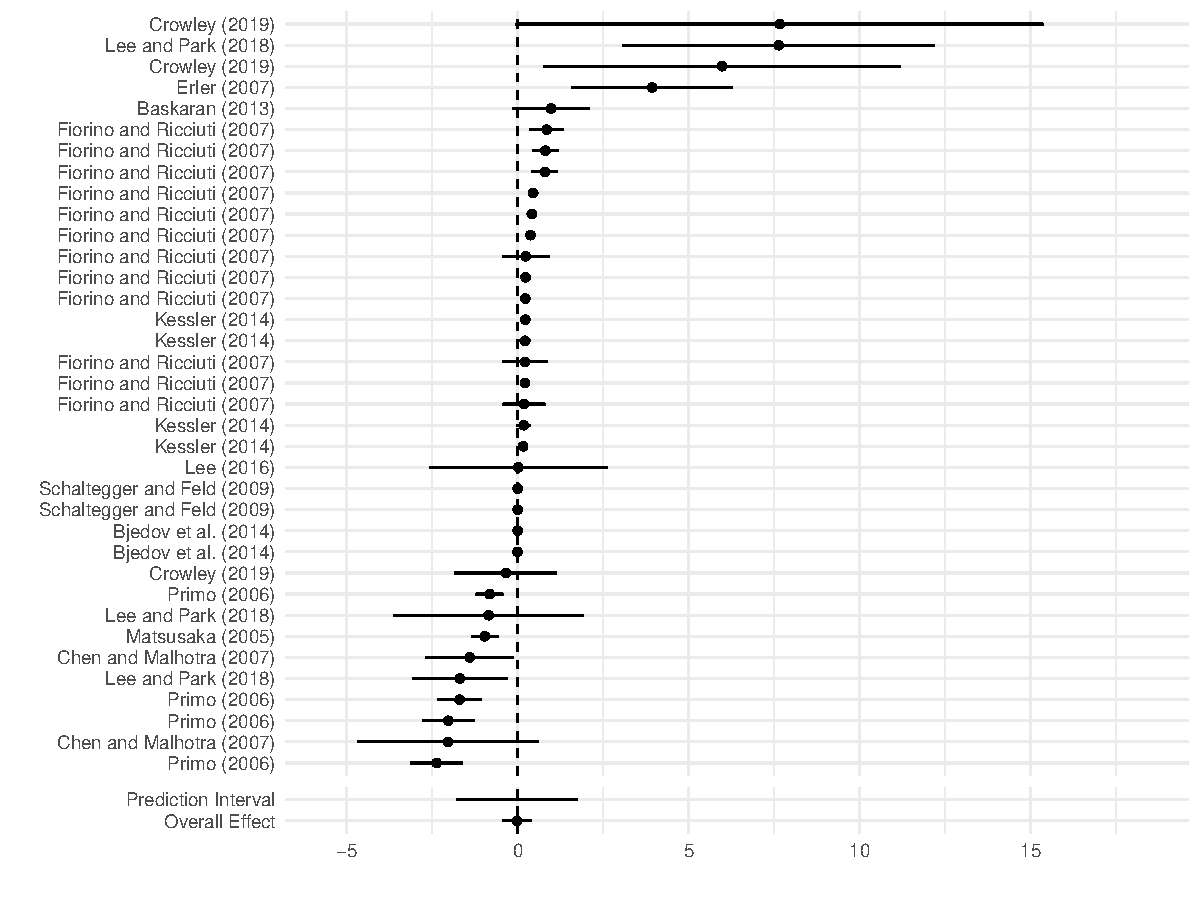
\includegraphics{appendixV5_files/figure-latex/unnamed-chunk-33-1.pdf}
\caption{Subgroup Analysis of (N) x (ExpPC), controlling by electoral
system}
\end{figure}

Therefore, we can see that the hypothesis that majoritarian systems
produce systematic positive effects was disproved. The majoritarian
systems in the sample had a random effects model estimate of -0.25,
while the random effects model in the non-majoritarian subgroup fitted a
value of 0.08. Both are non-significant, but they reassure us that the
absense of effect is not caused by pooling multiple types of electoral
systems.

\newpage

\hypertarget{pctgdp-x-n-1}{%
\subsubsection{PCTGDP x N}\label{pctgdp-x-n-1}}

This model fits the random effects for the percentage of GDP as public
expenditure as the main outcome, and the size of lower house as the main
treatment variable.

\begin{Shaded}
\begin{Highlighting}[]
\CommentTok{# Pooling effects analysis -- PCTGDP x N}
\NormalTok{aux <-}\StringTok{ }\NormalTok{fulldat }\OperatorTok
\StringTok{  }\KeywordTok{filter}\NormalTok{(indepvar2 }\OperatorTok{==}\StringTok{ 'N'}\NormalTok{,}
\NormalTok{         depvar2 }\OperatorTok{==}\StringTok{ 'PCTGDP'}\NormalTok{)}

\NormalTok{mod <-}\StringTok{ }\KeywordTok{metagen}\NormalTok{(coef, SE, }\DataTypeTok{data=}\NormalTok{aux, }
          \DataTypeTok{studlab=}\KeywordTok{paste}\NormalTok{(authoryear),}
          \DataTypeTok{comb.fixed =} \OtherTok{FALSE}\NormalTok{,}
          \DataTypeTok{comb.random =} \OtherTok{TRUE}\NormalTok{,}
          \DataTypeTok{method.tau =} \StringTok{"REML"}\NormalTok{,}
          \DataTypeTok{hakn =} \OtherTok{TRUE}\NormalTok{,}
          \DataTypeTok{prediction=}\OtherTok{TRUE}\NormalTok{,}
          \DataTypeTok{sm=}\StringTok{"SMD"}\NormalTok{)}
\NormalTok{mod}
\end{Highlighting}
\end{Shaded}

\begin{verbatim}
##                               SMD             95%-CI %W(random)
## Bjedov et al. (2014)      -0.0040 [-0.0432;  0.0352]        2.1
## Bjedov et al. (2014)      -0.0080 [-0.0472;  0.0312]        2.1
## Maldonado (2013)          -0.0609 [-0.0838; -0.0380]        3.6
## Mukherjee (2003)           0.0030 [ 0.0010;  0.0050]        5.6
## Mukherjee (2003)           0.0090 [ 0.0051;  0.0129]        5.5
## Mukherjee (2003)           0.0110 [ 0.0051;  0.0169]        5.4
## Mukherjee (2003)           0.0050 [-0.0009;  0.0109]        5.4
## Mukherjee (2003)           0.0400 [ 0.0380;  0.0420]        5.6
## Mukherjee (2003)           0.0300 [ 0.0280;  0.0320]        5.6
## Mukherjee (2003)           0.0100 [ 0.0061;  0.0139]        5.5
## Mukherjee (2003)           0.0200 [ 0.0122;  0.0278]        5.3
## Bradbury and Crain (2001)  0.0036 [ 0.0008;  0.0065]        5.6
## Bradbury and Crain (2001)  0.0005 [-0.0016;  0.0027]        5.6
## Bradbury and Crain (2001)  0.0169 [ 0.0131;  0.0208]        5.6
## Bradbury and Crain (2001)  0.0123 [ 0.0087;  0.0160]        5.6
## Ricciuti (2004)            0.0140 [-0.0095;  0.0375]        3.5
## Ricciuti (2004)           -0.0110 [-0.0286;  0.0066]        4.2
## Ricciuti (2004)            0.0070 [-0.0067;  0.0207]        4.7
## Ricciuti (2004)            0.0050 [-0.0126;  0.0226]        4.2
## Ricciuti (2004)            0.0050 [-0.0126;  0.0226]        4.2
## Ricciuti (2004)            0.0120 [-0.0017;  0.0257]        4.7
## 
## Number of studies combined: k = 21
## 
##                         SMD            95%-CI    t p-value
## Random effects model 0.0078 [-0.0003; 0.0160] 2.01  0.0579
## Prediction interval         [-0.0259; 0.0416]             
## 
## Quantifying heterogeneity:
##  tau^2 = 0.0002 [0.0002; 0.0007]; tau = 0.0156 [0.0136; 0.0261];
##  I^2 = 98.5% [98.2%; 98.7%]; H = 8.11 [7.40; 8.88]
## 
## Test of heterogeneity:
##        Q d.f.  p-value
##  1314.54   20 < 0.0001
## 
## Details on meta-analytical method:
## - Inverse variance method
## - Restricted maximum-likelihood estimator for tau^2
## - Q-profile method for confidence interval of tau^2 and tau
## - Hartung-Knapp adjustment for random effects model
\end{verbatim}

And the forest plot:

\begin{figure}
\centering
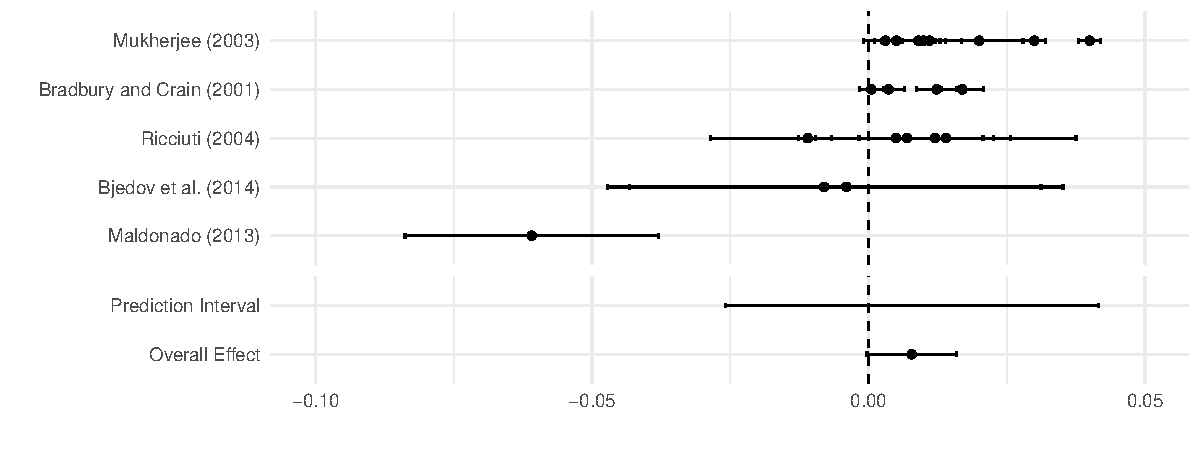
\includegraphics{appendixV5_files/figure-latex/unnamed-chunk-35-1.pdf}
\caption{Effect of lower houses size (N) on percentage of public
expenditure GDP (PCTGDP)}
\end{figure}

Highlights:

\begin{enumerate}
\def\labelenumi{\arabic{enumi}.}
\tightlist
\item
  The results are highly heterogeneous: \$I\^{}2 = \$ 98.48.
\item
  The Random effects modem SMD estimated is \$g = \$ 0.01 (\(SE =\)
  0.004).
\item
  The prediction interval ranges from -0.03 to 0.04. Therefore, it
  emcompasses zero.
\end{enumerate}

\newpage

\hypertarget{logexppc-x-n-1}{%
\subsubsection{logExpPC x N}\label{logexppc-x-n-1}}

This model estimates the Log of Per Capita Expenditure as the dependent
variable, and the number of lower house legislators as the treatment
variable.

\begin{Shaded}
\begin{Highlighting}[]
\CommentTok{# Pooling effects analysis -- logExpPC x N}
\NormalTok{aux <-}\StringTok{ }\NormalTok{fulldat }\OperatorTok
\StringTok{  }\KeywordTok{filter}\NormalTok{(indepvar2 }\OperatorTok{==}\StringTok{ 'N'}\NormalTok{,}
\NormalTok{         depvar2 }\OperatorTok{==}\StringTok{ 'logExpPC'}\NormalTok{)}

\NormalTok{mod <-}\StringTok{ }\KeywordTok{metagen}\NormalTok{(coef, SE, }\DataTypeTok{data=}\NormalTok{aux, }
          \DataTypeTok{studlab=}\KeywordTok{paste}\NormalTok{(authoryear),}
          \DataTypeTok{comb.fixed =} \OtherTok{FALSE}\NormalTok{,}
          \DataTypeTok{comb.random =} \OtherTok{TRUE}\NormalTok{,}
          \DataTypeTok{method.tau =} \StringTok{"REML"}\NormalTok{,}
          \DataTypeTok{hakn =} \OtherTok{TRUE}\NormalTok{,}
          \DataTypeTok{prediction=}\OtherTok{TRUE}\NormalTok{,}
          \DataTypeTok{sm=}\StringTok{"SMD"}\NormalTok{)}
\NormalTok{mod}
\end{Highlighting}
\end{Shaded}

\begin{verbatim}
##                              SMD             95%-CI %W(random)
## Lewis (2019)             -0.1740 [-0.2450; -0.1030]        6.6
## Höhmann (2017)           -0.0300 [-0.0496; -0.0104]        7.1
## Höhmann (2017)           -0.0300 [-0.0496; -0.0104]        7.1
## Höhmann (2017)           -0.0400 [-0.0792; -0.0008]        7.0
## Drew and Dollery (2017)   0.0770 [ 0.0221;  0.1319]        6.8
## Drew and Dollery (2017)   0.0310 [-0.0121;  0.0741]        6.9
## Pettersson-Lidbom (2012) -0.1590 [-0.2394; -0.0786]        6.4
## Pettersson-Lidbom (2012) -0.1470 [-0.2274; -0.0666]        6.4
## Pettersson-Lidbom (2012) -0.0900 [-0.1645; -0.0155]        6.5
## Pettersson-Lidbom (2012) -0.0810 [-0.1574; -0.0046]        6.5
## Pettersson-Lidbom (2012) -0.0880 [-0.1625; -0.0135]        6.5
## Pettersson-Lidbom (2012)  0.2100 [ 0.1649;  0.2551]        6.9
## Pettersson-Lidbom (2012)  0.1570 [ 0.0845;  0.2295]        6.5
## Pettersson-Lidbom (2012) -0.1990 [-0.2774; -0.1206]        6.4
## Pettersson-Lidbom (2012) -0.1690 [-0.2494; -0.0886]        6.4
## 
## Number of studies combined: k = 15
## 
##                          SMD            95%-CI     t p-value
## Random effects model -0.0463 [-0.1142; 0.0216] -1.46  0.1655
## Prediction interval          [-0.3105; 0.2178]              
## 
## Quantifying heterogeneity:
##  tau^2 = 0.0139 [0.0070; 0.0364]; tau = 0.1181 [0.0836; 0.1908];
##  I^2 = 93.8% [91.2%; 95.6%]; H = 4.00 [3.38; 4.75]
## 
## Test of heterogeneity:
##       Q d.f.  p-value
##  224.56   14 < 0.0001
## 
## Details on meta-analytical method:
## - Inverse variance method
## - Restricted maximum-likelihood estimator for tau^2
## - Q-profile method for confidence interval of tau^2 and tau
## - Hartung-Knapp adjustment for random effects model
\end{verbatim}

And the forest plot:

\begin{figure}
\centering
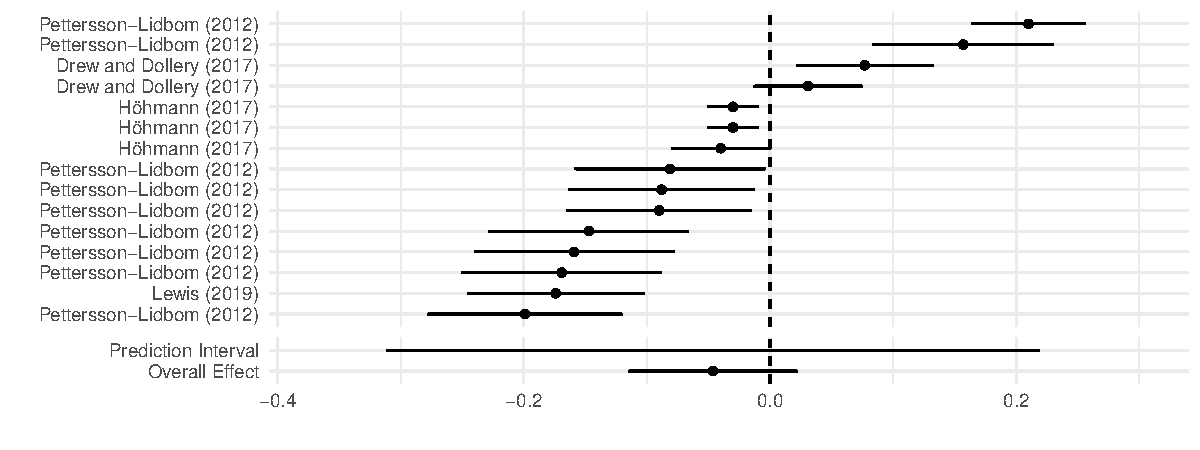
\includegraphics{appendixV5_files/figure-latex/unnamed-chunk-37-1.pdf}
\caption{Effect of lower houses size (N) on log of per capita
expenditure (logExpPC)}
\end{figure}

Highlights:

\begin{enumerate}
\def\labelenumi{\arabic{enumi}.}
\tightlist
\item
  The results are highly heterogeneous: \$I\^{}2 = \$ 93.77.
\item
  The Random effects modem SMD estimated is \$g = \$ -0.05 (\(SE =\)
  0.032).
\item
  The prediction interval ranges from -0.31 to 0.22. Therefore, it
  emcompasses zero.
\end{enumerate}

\newpage

\hypertarget{exppc-x-logn-1}{%
\subsubsection{ExpPC x logN}\label{exppc-x-logn-1}}

There were no studies that had per capita expenditure in the dependent
variable and log of lower house size in the treatment variable.

\hypertarget{pctgdp-x-logn-1}{%
\subsubsection{PCTGDP x logN}\label{pctgdp-x-logn-1}}

This meta-regression investigates the percentage of GDP as public
expenditure as the dependent variable and the log lower house size
(logN) as the treatment variable.

\begin{Shaded}
\begin{Highlighting}[]
\CommentTok{# Pooling effects analysis -- PCTGDP x logN}
\NormalTok{aux <-}\StringTok{ }\NormalTok{fulldat }\OperatorTok
\StringTok{  }\KeywordTok{filter}\NormalTok{(indepvar2 }\OperatorTok{==}\StringTok{ 'logN'}\NormalTok{,}
\NormalTok{         depvar2 }\OperatorTok{==}\StringTok{ 'PCTGDP'}\NormalTok{)}

\NormalTok{mod <-}\StringTok{ }\KeywordTok{metagen}\NormalTok{(coef, SE, }\DataTypeTok{data=}\NormalTok{aux, }
          \DataTypeTok{studlab=}\KeywordTok{paste}\NormalTok{(authoryear),}
          \DataTypeTok{comb.fixed =} \OtherTok{FALSE}\NormalTok{,}
          \DataTypeTok{comb.random =} \OtherTok{TRUE}\NormalTok{,}
          \DataTypeTok{method.tau =} \StringTok{"REML"}\NormalTok{,}
          \DataTypeTok{hakn =} \OtherTok{TRUE}\NormalTok{,}
          \DataTypeTok{prediction=}\OtherTok{TRUE}\NormalTok{,}
          \DataTypeTok{sm=}\StringTok{"SMD"}\NormalTok{)}
\NormalTok{mod}
\end{Highlighting}
\end{Shaded}

\begin{verbatim}
##                         SMD            95%-CI %W(random)
## Baqir (1999)         2.0660 [ 1.4887; 2.6433]       18.9
## Baqir (1999)         2.0120 [ 1.4235; 2.6005]       18.8
## Baqir (1999)         2.4680 [ 1.8817; 3.0543]       18.8
## Lledo (2003)        -4.6900 [-9.9427; 0.5627]        3.8
## Stein et al. (1998)  0.0109 [-0.0171; 0.0389]       19.8
## Stein et al. (1998)  0.0135 [-0.0102; 0.0372]       19.8
## 
## Number of studies combined: k = 6
## 
##                         SMD            95%-CI    t p-value
## Random effects model 1.0619 [-0.7256; 2.8493] 1.53  0.1873
## Prediction interval         [-3.0267; 5.1504]             
## 
## Quantifying heterogeneity:
##  tau^2 = 1.6850 [0.6497; 38.1618]; tau = 1.2981 [0.8060; 6.1775];
##  I^2 = 96.9% [95.2%; 98.1%]; H = 5.71 [4.55; 7.16]
## 
## Test of heterogeneity:
##       Q d.f.  p-value
##  163.00    5 < 0.0001
## 
## Details on meta-analytical method:
## - Inverse variance method
## - Restricted maximum-likelihood estimator for tau^2
## - Q-profile method for confidence interval of tau^2 and tau
## - Hartung-Knapp adjustment for random effects model
\end{verbatim}

And the forest plot:

\begin{figure}
\centering
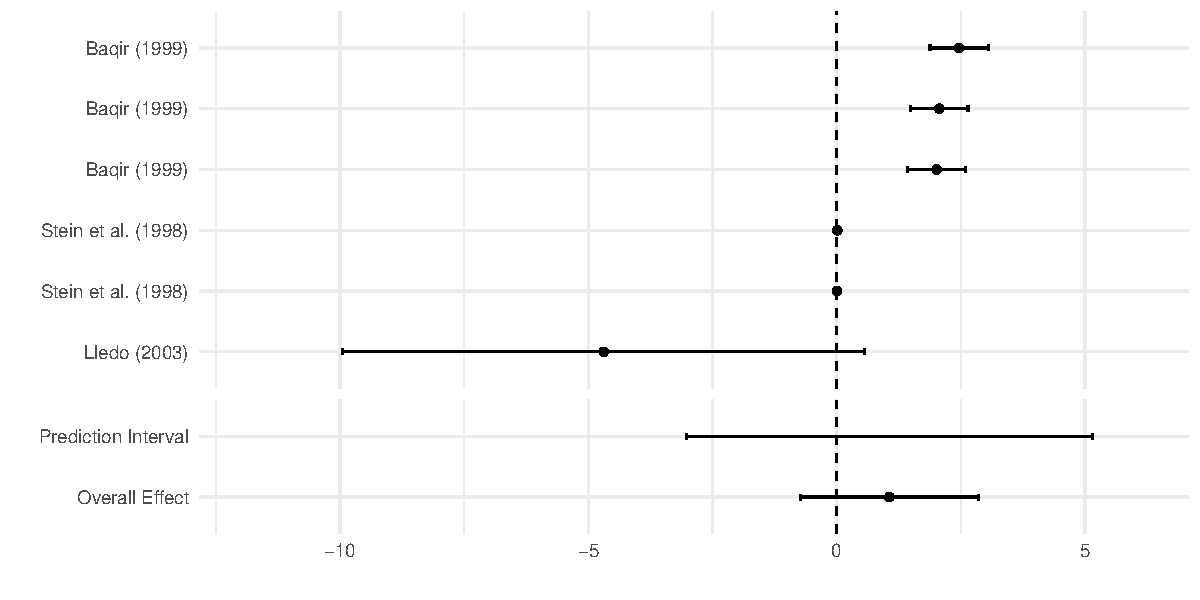
\includegraphics{appendixV5_files/figure-latex/unnamed-chunk-39-1.pdf}
\caption{Effect of log lower houses size (logN) on the GDP share of
public expenditure (PCTGDP)}
\end{figure}

Highlights:

\begin{enumerate}
\def\labelenumi{\arabic{enumi}.}
\tightlist
\item
  The results are highly heterogeneous: \$I\^{}2 = \$ 96.93.
\item
  The Random effects modem SMD estimated is \$g = \$ 1.06 (\(SE =\)
  0.695).
\item
  The prediction interval ranges from -3.03 to 5.15. Therefore, it
  emcompasses zero.
\end{enumerate}

\newpage

\hypertarget{logexppc-x-logn-1}{%
\subsubsection{logExpPC x logN}\label{logexppc-x-logn-1}}

In this specification, we study the log of per capita expenditure
(logExpPC) as a function of the log of lower house size (logN).

\begin{Shaded}
\begin{Highlighting}[]
\CommentTok{# Pooling effects analysis -- logExpPC x logN}
\NormalTok{aux <-}\StringTok{ }\NormalTok{fulldat }\OperatorTok
\StringTok{  }\KeywordTok{filter}\NormalTok{(indepvar2 }\OperatorTok{==}\StringTok{ 'logN'}\NormalTok{,}
\NormalTok{         depvar2 }\OperatorTok{==}\StringTok{ 'logExpPC'}\NormalTok{)}

\NormalTok{mod <-}\StringTok{ }\KeywordTok{metagen}\NormalTok{(coef, SE, }\DataTypeTok{data=}\NormalTok{aux, }
          \DataTypeTok{studlab=}\KeywordTok{paste}\NormalTok{(authoryear),}
          \DataTypeTok{comb.fixed =} \OtherTok{FALSE}\NormalTok{,}
          \DataTypeTok{comb.random =} \OtherTok{TRUE}\NormalTok{,}
          \DataTypeTok{method.tau =} \StringTok{"REML"}\NormalTok{,}
          \DataTypeTok{hakn =} \OtherTok{TRUE}\NormalTok{,}
          \DataTypeTok{prediction=}\OtherTok{TRUE}\NormalTok{,}
          \DataTypeTok{sm=}\StringTok{"SMD"}\NormalTok{)}
\NormalTok{mod}
\end{Highlighting}
\end{Shaded}

\begin{verbatim}
##                     SMD           95%-CI %W(random)
## MacDonald (2008) 0.1360 [0.0447; 0.2273]        7.9
## MacDonald (2008) 0.2319 [0.1322; 0.3316]        7.4
## MacDonald (2008) 0.1443 [0.0471; 0.2415]        7.6
## MacDonald (2008) 0.1594 [0.0667; 0.2521]        7.8
## MacDonald (2008) 0.2259 [0.1163; 0.3355]        6.9
## Baqir (2002)     0.1127 [0.0396; 0.1858]        9.1
## Baqir (2002)     0.2760 [0.2007; 0.3513]        8.9
## Baqir (2002)     0.3021 [0.2270; 0.3772]        8.9
## Baqir (2002)     0.3203 [0.2450; 0.3956]        8.9
## Baqir (1999)     0.3020 [0.2269; 0.3771]        8.9
## Baqir (1999)     0.2760 [0.2007; 0.3513]        8.9
## Baqir (1999)     0.2950 [0.2165; 0.3735]        8.7
## 
## Number of studies combined: k = 12
## 
##                         SMD           95%-CI     t  p-value
## Random effects model 0.2346 [0.1864; 0.2828] 10.71 < 0.0001
## Prediction interval         [0.0848; 0.3844]               
## 
## Quantifying heterogeneity:
##  tau^2 = 0.0040 [0.0011; 0.0145]; tau = 0.0636 [0.0335; 0.1203];
##  I^2 = 70.0% [45.6%; 83.4%]; H = 1.82 [1.36; 2.45]
## 
## Test of heterogeneity:
##      Q d.f. p-value
##  36.62   11  0.0001
## 
## Details on meta-analytical method:
## - Inverse variance method
## - Restricted maximum-likelihood estimator for tau^2
## - Q-profile method for confidence interval of tau^2 and tau
## - Hartung-Knapp adjustment for random effects model
\end{verbatim}

And the forest plot:

\begin{figure}
\centering
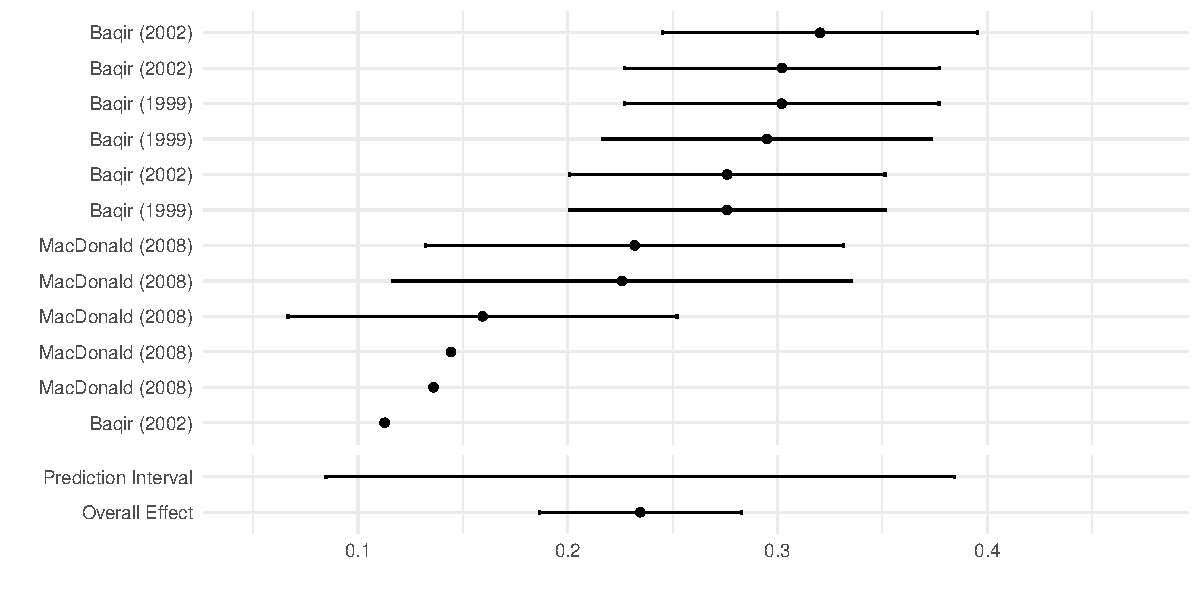
\includegraphics{appendixV5_files/figure-latex/unnamed-chunk-41-1.pdf}
\caption{Effect of log lower houses size (logN) on the log of per capita
government expenditure (logExpPC)}
\end{figure}

Highlights:

\begin{enumerate}
\def\labelenumi{\arabic{enumi}.}
\tightlist
\item
  The results are highly heterogeneous: \$I\^{}2 = \$ 69.96.
\item
  The Random effects modem SMD estimated is \$g = \$ 0.23 (\(SE =\)
  0.022). \textbf{This model is significant at the 10\% confidence
  level.}
\item
  The prediction interval ranges from 0.08 to 0.38. Therefore, it does
  not emcompasses zero.
\end{enumerate}

\newpage

\hypertarget{exppc-x-k-1}{%
\subsubsection{ExpPC x K}\label{exppc-x-k-1}}

Now we are investigating the upper house size (K). In this model, we
investigate the effect of upper house size on expenditure per capita
(ExpPC).

\begin{Shaded}
\begin{Highlighting}[]
\CommentTok{# Pooling effects analysis -- ExpPC x K}
\NormalTok{aux <-}\StringTok{ }\NormalTok{fulldat }\OperatorTok
\StringTok{  }\KeywordTok{filter}\NormalTok{(indepvar2 }\OperatorTok{==}\StringTok{ 'K'}\NormalTok{,}
\NormalTok{         depvar2 }\OperatorTok{==}\StringTok{ 'ExpPC'}\NormalTok{)}

\NormalTok{mod <-}\StringTok{ }\KeywordTok{metagen}\NormalTok{(coef, SE, }\DataTypeTok{data=}\NormalTok{aux, }
          \DataTypeTok{studlab=}\KeywordTok{paste}\NormalTok{(authoryear),}
          \DataTypeTok{comb.fixed =} \OtherTok{FALSE}\NormalTok{,}
          \DataTypeTok{comb.random =} \OtherTok{TRUE}\NormalTok{,}
          \DataTypeTok{method.tau =} \StringTok{"REML"}\NormalTok{,}
          \DataTypeTok{hakn =} \OtherTok{TRUE}\NormalTok{,}
          \DataTypeTok{prediction=}\OtherTok{TRUE}\NormalTok{,}
          \DataTypeTok{sm=}\StringTok{"SMD"}\NormalTok{)}
\NormalTok{mod}
\end{Highlighting}
\end{Shaded}

\begin{verbatim}
##                                    SMD              95%-CI %W(random)
## Crowley (2019)                  8.2100 [  0.2702; 16.1498]        4.8
## Crowley (2019)                  8.4230 [-27.1895; 44.0355]        0.4
## Crowley (2019)                  9.5940 [  2.1383; 17.0497]        5.1
## Lee and Park (2018)            19.7400 [  3.2645; 36.2155]        1.7
## Lee and Park (2018)            10.0600 [  2.2887; 17.8313]        4.9
## Lee and Park (2018)             9.0620 [-30.8821; 49.0061]        0.3
## Lee (2016)                     38.4400 [  0.7499; 76.1301]        0.4
## Lee (2016)                     37.8500 [  3.0214; 72.6786]        0.4
## Lee (2016)                     25.6100 [ -0.8103; 52.0303]        0.8
## Lee (2016)                      5.9960 [-19.6011; 31.5931]        0.8
## Lee (2016)                     25.5600 [ -0.8799; 51.9999]        0.8
## Lee (2016)                      4.6930 [-19.5126; 28.8986]        0.9
## Bradbury and Stephenson (2009)  0.6240 [  0.2295;  1.0185]       10.0
## Chen and Malhotra (2007)       26.0900 [ 11.4883; 40.6917]        2.1
## Chen and Malhotra (2007)        8.3000 [  3.6941; 12.9059]        7.3
## Chen and Malhotra (2007)        5.1400 [  0.1813; 10.0987]        7.0
## Chen and Malhotra (2007)        4.7800 [ -0.9039; 10.4639]        6.4
## Chen and Malhotra (2007)       20.3800 [  7.6990; 33.0610]        2.6
## Chen and Malhotra (2007)        4.8700 [  1.2833;  8.4567]        8.2
## Chen and Malhotra (2007)       26.7500 [  0.8589; 52.6411]        0.8
## Primo (2006)                    0.9700 [ -0.4804;  2.4204]        9.7
## Primo (2006)                    5.9000 [  2.6857;  9.1143]        8.5
## Primo (2006)                    5.7500 [  2.3593;  9.1407]        8.4
## Primo (2006)                    6.9600 [  2.6089; 11.3111]        7.6
## 
## Number of studies combined: k = 24
## 
##                         SMD             95%-CI    t  p-value
## Random effects model 7.2162 [ 4.4400;  9.9925] 5.38 < 0.0001
## Prediction interval         [-1.2217; 15.6542]              
## 
## Quantifying heterogeneity:
##  tau^2 = 14.7532 [5.4141; 111.2304]; tau = 3.8410 [2.3268; 10.5466];
##  I^2 = 77.7% [67.3%; 84.8%]; H = 2.12 [1.75; 2.57]
## 
## Test of heterogeneity:
##       Q d.f.  p-value
##  103.34   23 < 0.0001
## 
## Details on meta-analytical method:
## - Inverse variance method
## - Restricted maximum-likelihood estimator for tau^2
## - Q-profile method for confidence interval of tau^2 and tau
## - Hartung-Knapp adjustment for random effects model
\end{verbatim}

And the forest plot:

\begin{figure}
\centering
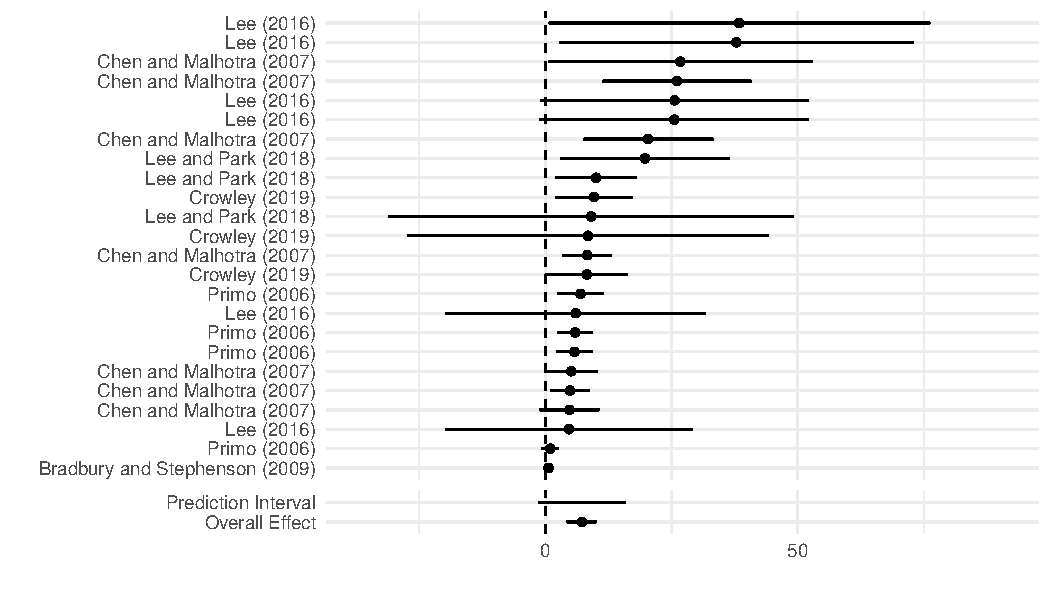
\includegraphics{appendixV5_files/figure-latex/unnamed-chunk-43-1.pdf}
\caption{Effect of upper house size (K) on the per capita government
expenditure (ExpPC)}
\end{figure}

Highlights:

\begin{enumerate}
\def\labelenumi{\arabic{enumi}.}
\tightlist
\item
  The results are highly heterogeneous: \$I\^{}2 = \$ 77.74.
\item
  The Random effects modem SMD estimated is \$g = \$ 7.22 (\(SE =\)
  1.342).
\item
  The prediction interval ranges from -1.22 to 15.65. Therefore, it
  emcompasses zero.
\end{enumerate}

\newpage

\hypertarget{pctgdp-x-k-1}{%
\subsubsection{PCTGDP x K}\label{pctgdp-x-k-1}}

This model looks into the effect of upper house size (K) on the public
expenditure share of the GDP (PCTGDP).

\begin{Shaded}
\begin{Highlighting}[]
\CommentTok{# Pooling effects analysis -- PCTGDP x K}
\NormalTok{aux <-}\StringTok{ }\NormalTok{fulldat }\OperatorTok
\StringTok{  }\KeywordTok{filter}\NormalTok{(indepvar2 }\OperatorTok{==}\StringTok{ 'K'}\NormalTok{,}
\NormalTok{         depvar2 }\OperatorTok{==}\StringTok{ 'PCTGDP'}\NormalTok{)}

\NormalTok{mod <-}\StringTok{ }\KeywordTok{metagen}\NormalTok{(coef, SE, }\DataTypeTok{data=}\NormalTok{aux, }
          \DataTypeTok{studlab=}\KeywordTok{paste}\NormalTok{(authoryear),}
          \DataTypeTok{comb.fixed =} \OtherTok{FALSE}\NormalTok{,}
          \DataTypeTok{comb.random =} \OtherTok{TRUE}\NormalTok{,}
          \DataTypeTok{method.tau =} \StringTok{"REML"}\NormalTok{,}
          \DataTypeTok{hakn =} \OtherTok{TRUE}\NormalTok{,}
          \DataTypeTok{prediction=}\OtherTok{TRUE}\NormalTok{,}
          \DataTypeTok{sm=}\StringTok{"SMD"}\NormalTok{)}
\NormalTok{mod}
\end{Highlighting}
\end{Shaded}

\begin{verbatim}
##                               SMD             95%-CI %W(random)
## Maldonado (2012)          -0.0400 [-0.0659; -0.0141]        5.7
## Bradbury and Crain (2001)  0.0126 [ 0.0010;  0.0243]        9.8
## Bradbury and Crain (2001)  0.0050 [ 0.0016;  0.0083]       11.8
## Bradbury and Crain (2001) -0.0113 [-0.0163; -0.0064]       11.5
## Bradbury and Crain (2001) -0.0056 [-0.0102; -0.0010]       11.6
## Ricciuti (2004)            0.0160 [-0.0075;  0.0395]        6.2
## Ricciuti (2004)            0.0210 [-0.0006;  0.0426]        6.7
## Ricciuti (2004)            0.0140 [-0.0036;  0.0316]        7.9
## Ricciuti (2004)            0.0030 [-0.0088;  0.0148]        9.7
## Ricciuti (2004)            0.0300 [-0.0210;  0.0810]        2.2
## Ricciuti (2004)            0.0300 [-0.0210;  0.0810]        2.2
## Ricciuti (2004)            0.0390 [-0.0022;  0.0802]        3.1
## Ricciuti (2004)            0.0127 [-0.0147;  0.0401]        5.3
## Ricciuti (2004)            0.0160 [-0.0075;  0.0395]        6.2
## 
## Number of studies combined: k = 14
## 
##                         SMD            95%-CI    t p-value
## Random effects model 0.0056 [-0.0042; 0.0155] 1.24  0.2376
## Prediction interval         [-0.0233; 0.0346]             
## 
## Quantifying heterogeneity:
##  tau^2 = 0.0002 [0.0001; 0.0008]; tau = 0.0125 [0.0109; 0.0279];
##  I^2 = 80.0% [67.3%; 87.8%]; H = 2.24 [1.75; 2.86]
## 
## Test of heterogeneity:
##      Q d.f.  p-value
##  65.02   13 < 0.0001
## 
## Details on meta-analytical method:
## - Inverse variance method
## - Restricted maximum-likelihood estimator for tau^2
## - Q-profile method for confidence interval of tau^2 and tau
## - Hartung-Knapp adjustment for random effects model
\end{verbatim}

And the forest plot:

\begin{figure}
\centering
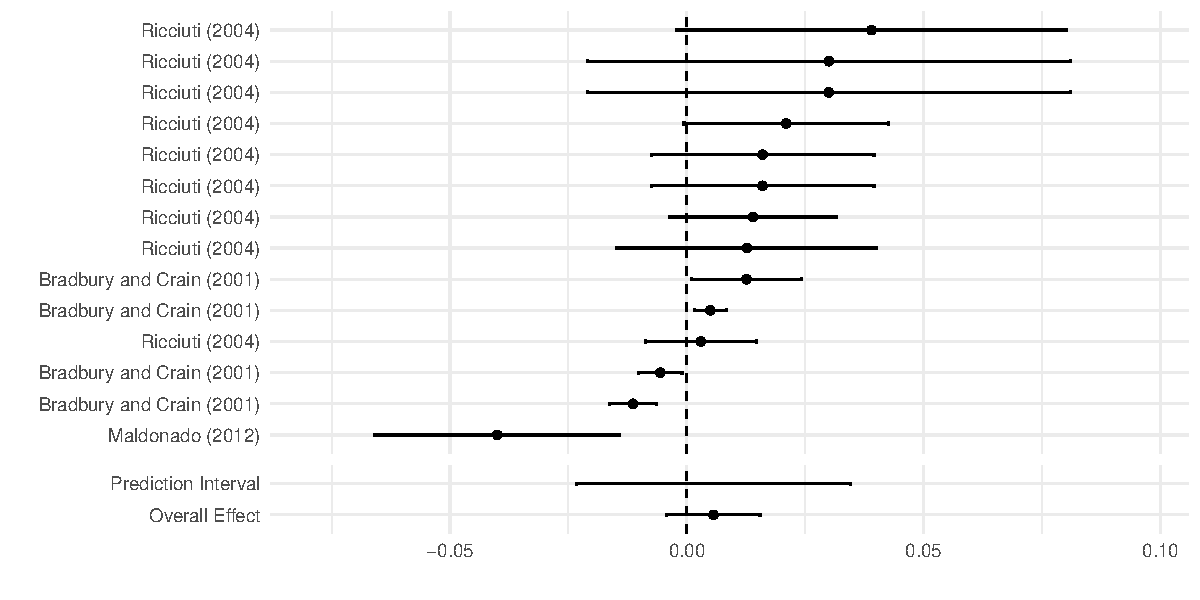
\includegraphics{appendixV5_files/figure-latex/unnamed-chunk-45-1.pdf}
\caption{Effect of upper house size (K) on the public expenditure share
of the GDP (PCTGDP)}
\end{figure}

Highlights:

\begin{enumerate}
\def\labelenumi{\arabic{enumi}.}
\tightlist
\item
  The results are highly heterogeneous: \$I\^{}2 = \$ 80.01.
\item
  The Random effects modem SMD estimated is \$g = \$ 0.01 (\(SE =\)
  0.005).
\item
  The prediction interval ranges from -0.02 to 0.03. Therefore, it
  emcompasses zero.
\end{enumerate}

\hypertarget{logexppc-x-k-1}{%
\subsubsection{logExpPC x K}\label{logexppc-x-k-1}}

No studies related the log of per capita expenditure with the size of
upper house (K).


\includegraphics{appendixV5_files/figure-latex/unnamed-chunk-46-2.pdf}
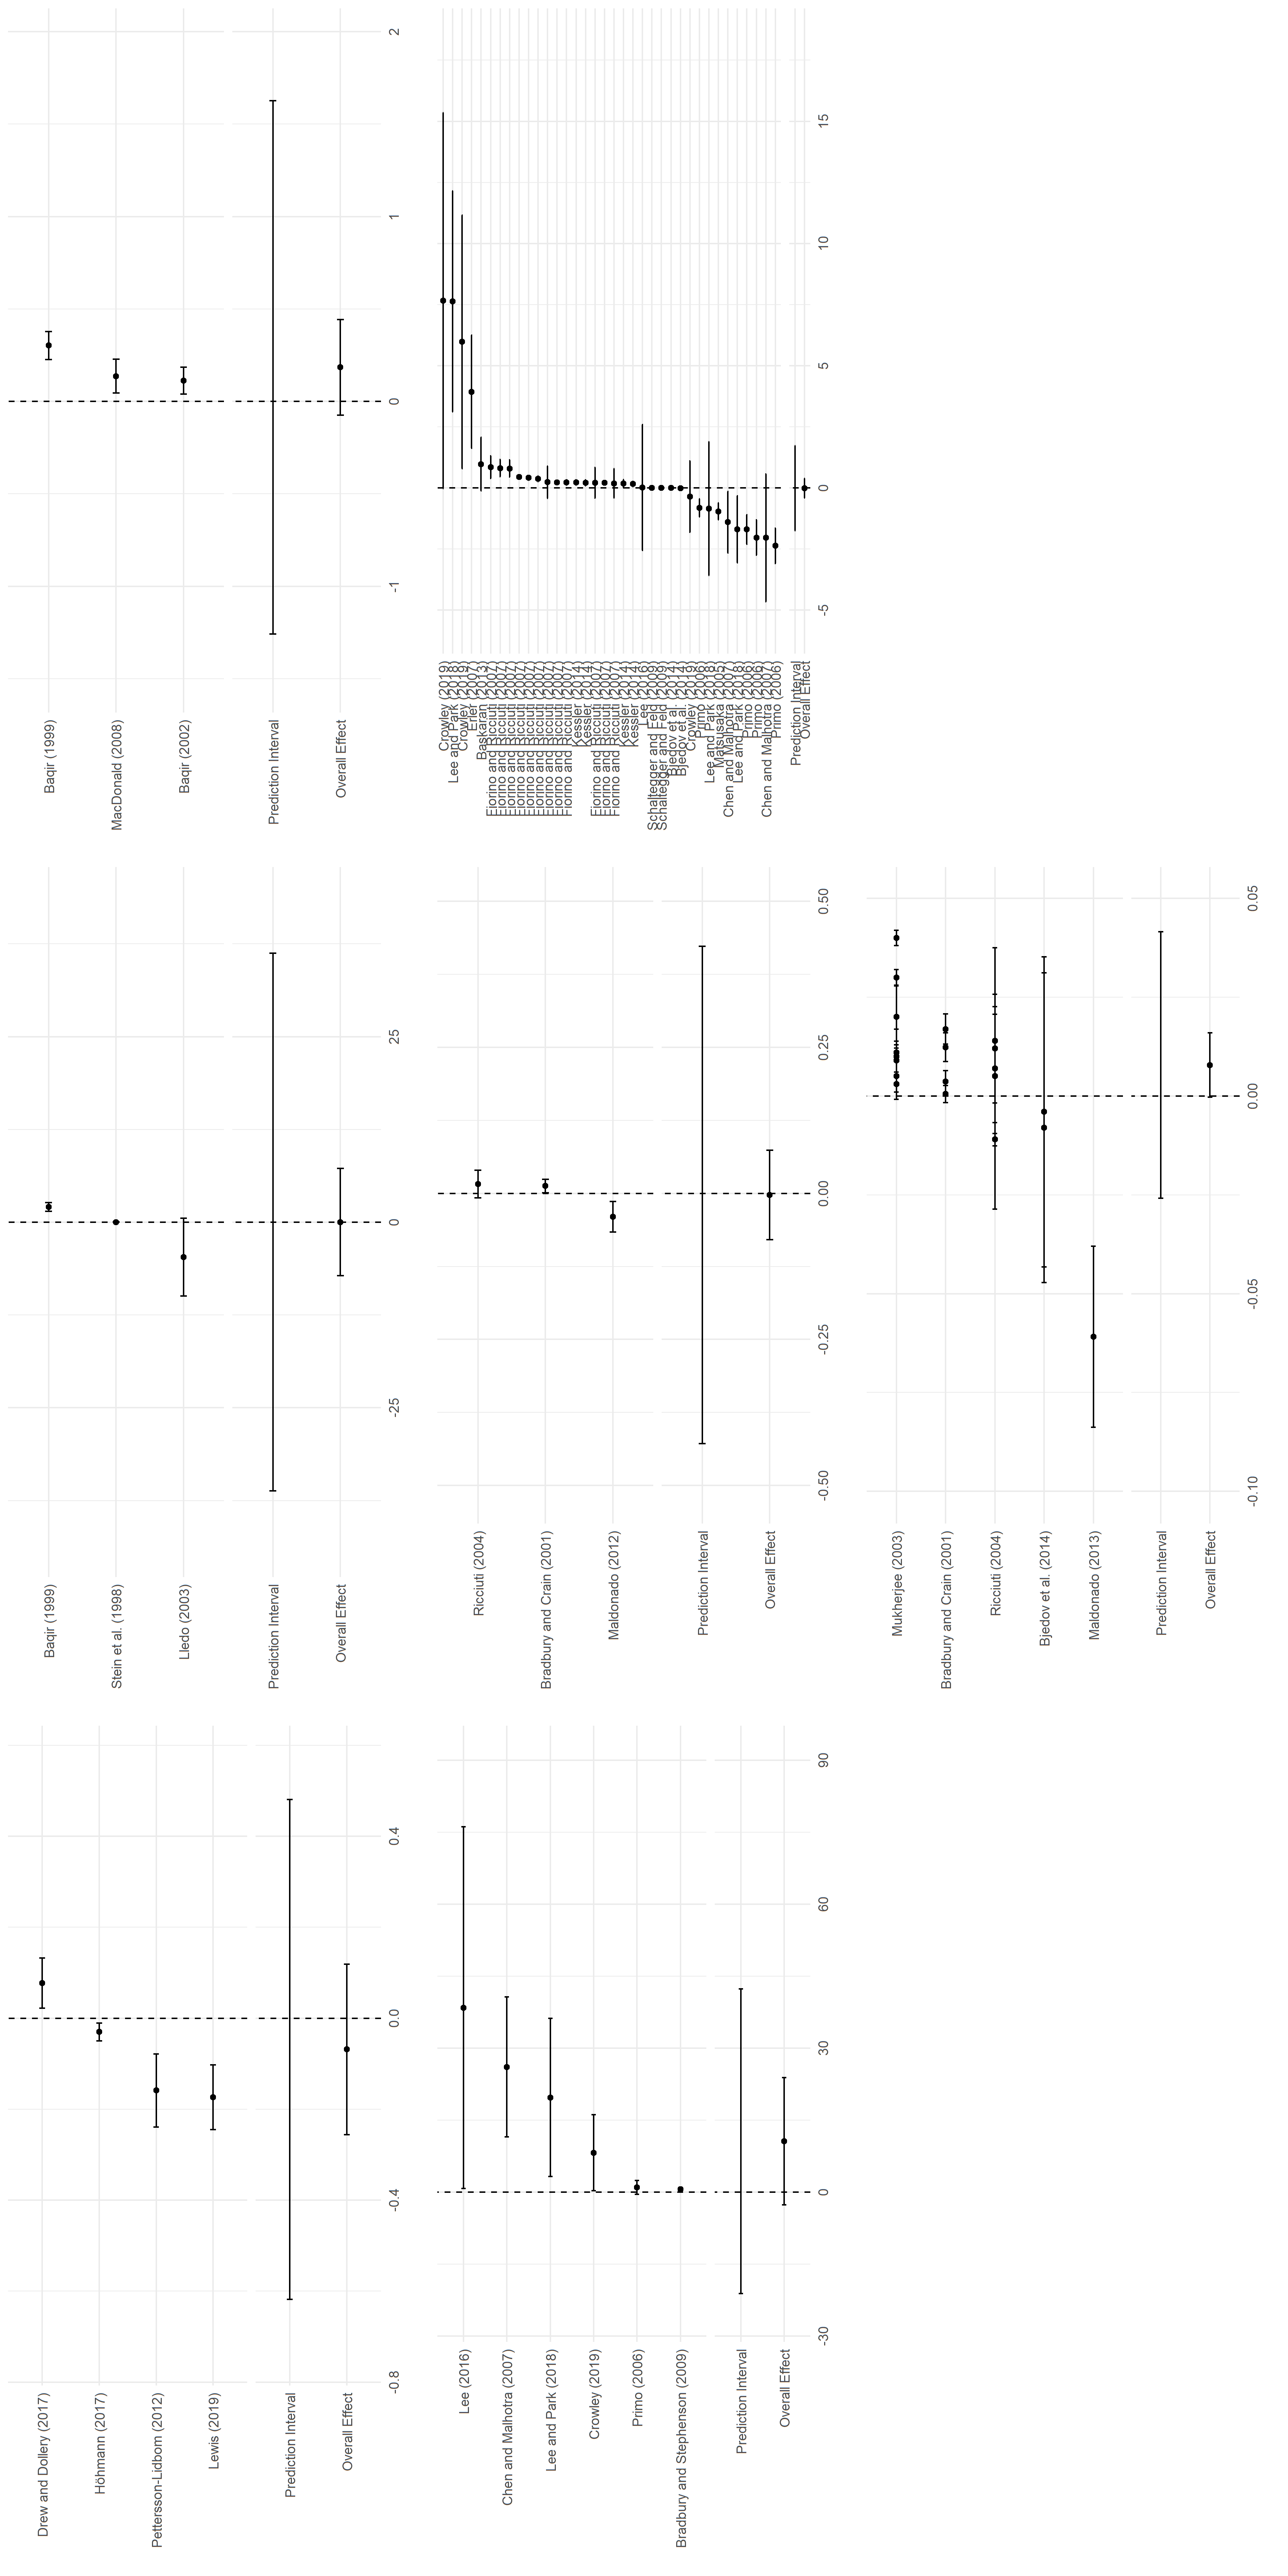
\includegraphics[width=49.21in]{appendixV5_files/figure-latex/unnamed-chunk-46-1}

\newpage

\hypertarget{meta-regressions}{%
\subsection{Meta-regressions}\label{meta-regressions}}

\hypertarget{meta-regressions-for-expenditure-as-a-percentage-of-the-gdp}{%
\subsubsection{Meta-regressions for Expenditure as a Percentage of the
GDP}\label{meta-regressions-for-expenditure-as-a-percentage-of-the-gdp}}

\begin{Shaded}
\begin{Highlighting}[]
\KeywordTok{summary}\NormalTok{(mod)}
\end{Highlighting}
\end{Shaded}

\begin{verbatim}
## 
## Mixed-Effects Model (k = 11; tau^2 estimator: REML)
## 
##   logLik  deviance       AIC       BIC      AICc 
##   7.0993  -14.1987    5.8013   -7.2672  225.8013   
## 
## tau^2 (estimated amount of residual heterogeneity):     0 (SE = 0.0001)
## tau (square root of estimated tau^2 value):             0
## I^2 (residual heterogeneity / unaccounted variability): 0.00%
## H^2 (unaccounted variability / sampling variability):   1.00
## R^2 (amount of heterogeneity accounted for):            100.00%
## 
## Test for Residual Heterogeneity:
## QE(df = 2) = 0.5965, p-val = 0.7421
## 
## Test of Moderators (coefficients 2:9):
## F(df1 = 8, df2 = 2) = 40.7363, p-val = 0.0242
## 
## Model Results:
## 
##                           estimate      se      tval    pval     ci.lb    ci.ub 
## intrcpt                     7.3697  1.7616    4.1835  0.0527   -0.2099  14.9493 
## indepvar2N                 -0.0094  0.0030   -3.1174  0.0893   -0.0223   0.0036 
## indepvar2logN              -4.7067  1.4637   -3.2156  0.0846  -11.0045   1.5912 
## year                       -0.0003  0.0005   -0.6899  0.5615   -0.0024   0.0017 
## publishedNo                 0.0633  0.0078    8.1139  0.0149    0.0297   0.0969 
## elecsys2Non-Majoritarian   -2.0554  0.1611  -12.7621  0.0061   -2.7484  -1.3625 
## methodPANEL                 0.0556  0.0071    7.7913  0.0161    0.0249   0.0864 
## agglevelStates             -4.6992  1.4637   -3.2106  0.0848  -10.9969   1.5984 
## location2World             -4.6959  1.4637   -3.2082  0.0850  -10.9937   1.6019 
##  
## intrcpt                    . 
## indepvar2N                 . 
## indepvar2logN              . 
## year 
## publishedNo                * 
## elecsys2Non-Majoritarian  ** 
## methodPANEL                * 
## agglevelStates             . 
## location2World             . 
## 
## ---
## Signif. codes:  0 '***' 0.001 '**' 0.01 '*' 0.05 '.' 0.1 ' ' 1
\end{verbatim}

As we have considerable heterogeneity in our sample, we run a
permutation test to ensure the validity of our estimates. The results
follow below.

\begin{verbatim}
## Error in rma.uni(x$yi, x$vi, weights = x$weights, mods = cbind(X[sample(x$k),  : 
##   Fisher scoring algorithm did not converge. See 'help(rma)' for possible remedies.
## Error in rma.uni(x$yi, x$vi, weights = x$weights, mods = cbind(X[sample(x$k),  : 
##   Fisher scoring algorithm did not converge. See 'help(rma)' for possible remedies.
\end{verbatim}

\begin{verbatim}
## 
## Test of Moderators (coefficients 2:9):
## F(df1 = 8, df2 = 2) = 40.7363, p-val* = 0.0130
## 
## Model Results:
## 
##                           estimate      se      tval   pval*     ci.lb    ci.ub 
## intrcpt                     7.3697  1.7616    4.1835  0.0360   -0.2099  14.9493 
## indepvar2N                 -0.0094  0.0030   -3.1174  0.0190   -0.0223   0.0036 
## indepvar2logN              -4.7067  1.4637   -3.2156  0.2010  -11.0045   1.5912 
## year                       -0.0003  0.0005   -0.6899  0.4350   -0.0024   0.0017 
## publishedNo                 0.0633  0.0078    8.1139  0.0140    0.0297   0.0969 
## elecsys2Non-Majoritarian   -2.0554  0.1611  -12.7621  0.0090   -2.7484  -1.3625 
## methodPANEL                 0.0556  0.0071    7.7913  0.0140    0.0249   0.0864 
## agglevelStates             -4.6992  1.4637   -3.2106  0.2170  -10.9969   1.5984 
## location2World             -4.6959  1.4637   -3.2082  0.2790  -10.9937   1.6019 
##  
## intrcpt                    * 
## indepvar2N                 * 
## indepvar2logN 
## year 
## publishedNo                * 
## elecsys2Non-Majoritarian  ** 
## methodPANEL                * 
## agglevelStates 
## location2World 
## 
## ---
## Signif. codes:  0 '***' 0.001 '**' 0.01 '*' 0.05 '.' 0.1 ' ' 1
\end{verbatim}

We have the following results for the meta-regressions of Expenditure
Per Capita:

\begin{enumerate}
\def\labelenumi{\arabic{enumi}.}
\tightlist
\item
  Compared with \texttt{K}, models with \texttt{N} and \texttt{logN}
  find significantly negative coefficients.
\item
  Year has null effect.
\item
  Unpublished papers tend to have higher coefficients than published
  papers.
\item
  Passing from \texttt{Majoritarian} to \texttt{Non-Majoritarian},
  decreases significantly the effects found in our models.
\item
  In terms of the modeling, passing from \texttt{OLS} to \texttt{PANEL}
  increases the detected effects.
\item
  When passing from \texttt{Local} to \texttt{State} or \texttt{World}
  levels, it decreases the detected effect size.
\end{enumerate}

Below we also run the meta-regressions adding all coefficients in the
papers. The results follow below:

\begin{Shaded}
\begin{Highlighting}[]
\KeywordTok{summary}\NormalTok{(mod)}
\end{Highlighting}
\end{Shaded}

\begin{verbatim}
## 
## Mixed-Effects Model (k = 41; tau^2 estimator: REML)
## 
##    logLik   deviance        AIC        BIC       AICc 
##   89.1145  -178.2290  -158.2290  -143.5716  -147.7528   
## 
## tau^2 (estimated amount of residual heterogeneity):     0.0001 (SE = 0.0000)
## tau (square root of estimated tau^2 value):             0.0102
## I^2 (residual heterogeneity / unaccounted variability): 94.05%
## H^2 (unaccounted variability / sampling variability):   16.81
## R^2 (amount of heterogeneity accounted for):            99.92%
## 
## Test for Residual Heterogeneity:
## QE(df = 32) = 1001.8067, p-val < .0001
## 
## Test of Moderators (coefficients 2:9):
## F(df1 = 8, df2 = 32) = 29.7201, p-val < .0001
## 
## Model Results:
## 
##                           estimate      se      tval    pval     ci.lb    ci.ub 
## intrcpt                    -5.3830  5.8900   -0.9139  0.3676  -17.3805   6.6145 
## indepvar2N                 -0.0014  0.0048   -0.2945  0.7703   -0.0112   0.0084 
## indepvar2logN              -4.6069  2.4363   -1.8909  0.0677   -9.5696   0.3558 
## year                        0.0060  0.0027    2.2730  0.0299    0.0006   0.0114 
## publishedNo                 0.1130  0.0251    4.5060  <.0001    0.0619   0.1641 
## elecsys2Non-Majoritarian   -2.1629  0.1568  -13.7904  <.0001   -2.4823  -1.8434 
## methodPANEL                 0.1252  0.0304    4.1232  0.0002    0.0633   0.1870 
## agglevelStates             -4.7325  2.4361   -1.9426  0.0609   -9.6947   0.2298 
## location2World             -4.6443  2.4362   -1.9064  0.0656   -9.6067   0.3181 
##  
## intrcpt 
## indepvar2N 
## indepvar2logN               . 
## year                        * 
## publishedNo               *** 
## elecsys2Non-Majoritarian  *** 
## methodPANEL               *** 
## agglevelStates              . 
## location2World              . 
## 
## ---
## Signif. codes:  0 '***' 0.001 '**' 0.01 '*' 0.05 '.' 0.1 ' ' 1
\end{verbatim}

\begin{Shaded}
\begin{Highlighting}[]
\KeywordTok{permutest}\NormalTok{(mod, }\DataTypeTok{progbar =}\NormalTok{ F)}
\end{Highlighting}
\end{Shaded}

\begin{verbatim}
## 
## Test of Moderators (coefficients 2:9):
## F(df1 = 8, df2 = 32) = 29.7201, p-val* = 0.0010
## 
## Model Results:
## 
##                           estimate      se      tval   pval*     ci.lb    ci.ub 
## intrcpt                    -5.3830  5.8900   -0.9139  0.2800  -17.3805   6.6145 
## indepvar2N                 -0.0014  0.0048   -0.2945  0.7390   -0.0112   0.0084 
## indepvar2logN              -4.6069  2.4363   -1.8909  0.0910   -9.5696   0.3558 
## year                        0.0060  0.0027    2.2730  0.0090    0.0006   0.0114 
## publishedNo                 0.1130  0.0251    4.5060  0.0020    0.0619   0.1641 
## elecsys2Non-Majoritarian   -2.1629  0.1568  -13.7904  0.0010   -2.4823  -1.8434 
## methodPANEL                 0.1252  0.0304    4.1232  0.0020    0.0633   0.1870 
## agglevelStates             -4.7325  2.4361   -1.9426  0.0840   -9.6947   0.2298 
## location2World             -4.6443  2.4362   -1.9064  0.0950   -9.6067   0.3181 
##  
## intrcpt 
## indepvar2N 
## indepvar2logN               . 
## year                       ** 
## publishedNo                ** 
## elecsys2Non-Majoritarian  *** 
## methodPANEL                ** 
## agglevelStates              . 
## location2World              . 
## 
## ---
## Signif. codes:  0 '***' 0.001 '**' 0.01 '*' 0.05 '.' 0.1 ' ' 1
\end{verbatim}

For all the coefficients, we have the following results:

\begin{enumerate}
\def\labelenumi{\arabic{enumi}.}
\tightlist
\item
  Compared with \texttt{K}, models with \texttt{N} and \texttt{logN}
  tend to have significantly negative coefficients.
\item
  Year has a positive effect: the younger the publication, the higher
  the detected coefficient.
\item
  Unpublished papers tend to have higher coefficients than published
  papers.
\item
  Passing from \texttt{Majoritarian} to \texttt{Non-Majoritarian},
  decreases significantly the effects found in our models.
\item
  In terms of the modeling, passing from \texttt{OLS} to \texttt{PANEL}
  increases the detected effects.
\item
  When passing from \texttt{Local} to \texttt{State} or \texttt{World}
  levels, it decreases the detected effect size.
\end{enumerate}

\hypertarget{meta-regressions-for-expenditure-per-capita}{%
\subsubsection{Meta-regressions for Expenditure Per
Capita}\label{meta-regressions-for-expenditure-per-capita}}

\begin{Shaded}
\begin{Highlighting}[]
\KeywordTok{summary}\NormalTok{(mod)}
\end{Highlighting}
\end{Shaded}

\begin{verbatim}
## 
## Mixed-Effects Model (k = 18; tau^2 estimator: REML)
## 
##   logLik  deviance       AIC       BIC      AICc 
## -34.6251   69.2502   85.2502   88.4333  157.2502   
## 
## tau^2 (estimated amount of residual heterogeneity):     1.8429 (SE = 1.2361)
## tau (square root of estimated tau^2 value):             1.3575
## I^2 (residual heterogeneity / unaccounted variability): 95.05%
## H^2 (unaccounted variability / sampling variability):   20.21
## R^2 (amount of heterogeneity accounted for):            0.00%
## 
## Test for Residual Heterogeneity:
## QE(df = 11) = 45.4940, p-val < .0001
## 
## Test of Moderators (coefficients 2:7):
## F(df1 = 6, df2 = 11) = 0.3429, p-val = 0.8998
## 
## Model Results:
## 
##                            estimate        se     tval    pval      ci.lb 
## intrcpt                   -104.0701  318.9300  -0.3263  0.7503  -806.0302 
## indepvar2N                  -2.9238    2.0932  -1.3968  0.1900    -7.5309 
## year                         0.0525    0.1586   0.3308  0.7470    -0.2967 
## elecsys2Non-Majoritarian     0.3458    1.5533   0.2226  0.8279    -3.0730 
## methodPANEL                  1.4571    2.2376   0.6512  0.5283    -3.4679 
## methodIV                     1.4936    2.6675   0.5599  0.5868    -4.3776 
## agglevelStates              -0.0915    2.4255  -0.0377  0.9706    -5.4299 
##                              ci.ub 
## intrcpt                   597.8900    
## indepvar2N                  1.6834    
## year                        0.4017    
## elecsys2Non-Majoritarian    3.7645    
## methodPANEL                 6.3821    
## methodIV                    7.3648    
## agglevelStates              5.2470    
## 
## ---
## Signif. codes:  0 '***' 0.001 '**' 0.01 '*' 0.05 '.' 0.1 ' ' 1
\end{verbatim}

As we have considerable heterogeneity in our sample, we run a
permutation test to ensure the validity of our estimates. The results
follow below.

\begin{verbatim}
## Error in rma.uni(x$yi, x$vi, weights = x$weights, mods = cbind(X[sample(x$k),  : 
##   Fisher scoring algorithm did not converge. See 'help(rma)' for possible remedies.
## Error in rma.uni(x$yi, x$vi, weights = x$weights, mods = cbind(X[sample(x$k),  : 
##   Fisher scoring algorithm did not converge. See 'help(rma)' for possible remedies.
## Error in rma.uni(x$yi, x$vi, weights = x$weights, mods = cbind(X[sample(x$k),  : 
##   Fisher scoring algorithm did not converge. See 'help(rma)' for possible remedies.
## Error in rma.uni(x$yi, x$vi, weights = x$weights, mods = cbind(X[sample(x$k),  : 
##   Fisher scoring algorithm did not converge. See 'help(rma)' for possible remedies.
\end{verbatim}

\begin{verbatim}
## 
## Test of Moderators (coefficients 2:7):
## F(df1 = 6, df2 = 11) = 0.3429, p-val* = 0.5900
## 
## Model Results:
## 
##                            estimate        se     tval   pval*      ci.lb 
## intrcpt                   -104.0701  318.9300  -0.3263  0.6300  -806.0302 
## indepvar2N                  -2.9238    2.0932  -1.3968  0.0650    -7.5309 
## year                         0.0525    0.1586   0.3308  0.6270    -0.2967 
## elecsys2Non-Majoritarian     0.3458    1.5533   0.2226  0.7180    -3.0730 
## methodPANEL                  1.4571    2.2376   0.6512  0.3330    -3.4679 
## methodIV                     1.4936    2.6675   0.5599  0.4380    -4.3776 
## agglevelStates              -0.0915    2.4255  -0.0377  0.9440    -5.4299 
##                              ci.ub 
## intrcpt                   597.8900    
## indepvar2N                  1.6834  . 
## year                        0.4017    
## elecsys2Non-Majoritarian    3.7645    
## methodPANEL                 6.3821    
## methodIV                    7.3648    
## agglevelStates              5.2470    
## 
## ---
## Signif. codes:  0 '***' 0.001 '**' 0.01 '*' 0.05 '.' 0.1 ' ' 1
\end{verbatim}

We have the following results for the meta-regressions of Expenditure
Per Capita:

\begin{enumerate}
\def\labelenumi{\arabic{enumi}.}
\tightlist
\item
  Compared with \texttt{K}, models with \texttt{N} tend to detect
  significantly smaller effects.
\item
  Year has null effect.
\item
  Passing the electoral rules from \texttt{Majoritarian} to
  \texttt{Non-Majoritarian}, increases significantly the per capita
  expenditure found in our models.
\item
  In terms of the modeling, passing from \texttt{OLS} to \texttt{PANEL}
  or \texttt{IV} increases the detected effects.
\item
  When passing from \texttt{Local} to \texttt{State} level, decreases
  the detected effects.
\end{enumerate}

Below we also run the meta-regressions adding all coefficients in the
papers. The results follow below:

\begin{Shaded}
\begin{Highlighting}[]
\KeywordTok{summary}\NormalTok{(mod)}
\end{Highlighting}
\end{Shaded}

\begin{verbatim}
## 
## Mixed-Effects Model (k = 60; tau^2 estimator: REML)
## 
##    logLik   deviance        AIC        BIC       AICc 
## -141.1228   282.2456   298.2456   314.0079   301.5183   
## 
## tau^2 (estimated amount of residual heterogeneity):     1.7264 (SE = 0.4944)
## tau (square root of estimated tau^2 value):             1.3139
## I^2 (residual heterogeneity / unaccounted variability): 99.80%
## H^2 (unaccounted variability / sampling variability):   500.07
## R^2 (amount of heterogeneity accounted for):            39.21%
## 
## Test for Residual Heterogeneity:
## QE(df = 53) = 325.8548, p-val < .0001
## 
## Test of Moderators (coefficients 2:7):
## F(df1 = 6, df2 = 53) = 5.9441, p-val < .0001
## 
## Model Results:
## 
##                            estimate        se     tval    pval      ci.lb 
## intrcpt                   -296.9072  166.6870  -1.7812  0.0806  -631.2389 
## indepvar2N                  -5.4468    0.9692  -5.6201  <.0001    -7.3907 
## year                         0.1503    0.0830   1.8117  0.0757    -0.0161 
## elecsys2Non-Majoritarian     1.0236    0.7701   1.3293  0.1894    -0.5209 
## methodPANEL                 -0.1422    0.8136  -0.1747  0.8620    -1.7739 
## methodIV                     0.1907    0.8223   0.2319  0.8175    -1.4587 
## agglevelStates              -0.2008    1.0049  -0.1998  0.8424    -2.2164 
##                             ci.ub 
## intrcpt                   37.4245    . 
## indepvar2N                -3.5029  *** 
## year                       0.3167    . 
## elecsys2Non-Majoritarian   2.5682      
## methodPANEL                1.4896      
## methodIV                   1.8401      
## agglevelStates             1.8149      
## 
## ---
## Signif. codes:  0 '***' 0.001 '**' 0.01 '*' 0.05 '.' 0.1 ' ' 1
\end{verbatim}

\begin{Shaded}
\begin{Highlighting}[]
\KeywordTok{permutest}\NormalTok{(mod, }\DataTypeTok{progbar =}\NormalTok{ F)}
\end{Highlighting}
\end{Shaded}

\begin{verbatim}
## 
## Test of Moderators (coefficients 2:7):
## F(df1 = 6, df2 = 53) = 5.9441, p-val* = 0.0010
## 
## Model Results:
## 
##                            estimate        se     tval   pval*      ci.lb 
## intrcpt                   -296.9072  166.6870  -1.7812  0.0170  -631.2389 
## indepvar2N                  -5.4468    0.9692  -5.6201  0.0010    -7.3907 
## year                         0.1503    0.0830   1.8117  0.0150    -0.0161 
## elecsys2Non-Majoritarian     1.0236    0.7701   1.3293  0.0730    -0.5209 
## methodPANEL                 -0.1422    0.8136  -0.1747  0.7990    -1.7739 
## methodIV                     0.1907    0.8223   0.2319  0.7700    -1.4587 
## agglevelStates              -0.2008    1.0049  -0.1998  0.7990    -2.2164 
##                             ci.ub 
## intrcpt                   37.4245    * 
## indepvar2N                -3.5029  *** 
## year                       0.3167    * 
## elecsys2Non-Majoritarian   2.5682    . 
## methodPANEL                1.4896      
## methodIV                   1.8401      
## agglevelStates             1.8149      
## 
## ---
## Signif. codes:  0 '***' 0.001 '**' 0.01 '*' 0.05 '.' 0.1 ' ' 1
\end{verbatim}

With all coefficients, the results of the effect sizes on the
Expenditure Per Capita Regressions are the following:

\begin{enumerate}
\def\labelenumi{\arabic{enumi}.}
\tightlist
\item
  Compared with \texttt{K}, models with \texttt{N} tend to detect
  significantly smaller effects.
\item
  Year has now a positive effect on coefficient sizes.
\item
  Passing the electoral rules from \texttt{Majoritarian} to
  \texttt{Non-Majoritarian}, increases significantly the effects on per
  capita expenditure found in our models.
\item
  In terms of the modeling, passing from \texttt{OLS} to \texttt{PANEL}
  decreases the detected effects.
\item
  All other coeffients were not significant.
\end{enumerate}

\hypertarget{meta-regressions-for-the-log-of-expenditure-per-capita}{%
\subsubsection{Meta-regressions for the Log of Expenditure Per
Capita}\label{meta-regressions-for-the-log-of-expenditure-per-capita}}

\begin{Shaded}
\begin{Highlighting}[]
\KeywordTok{summary}\NormalTok{(mod)}
\end{Highlighting}
\end{Shaded}

\begin{verbatim}
## 
## Mixed-Effects Model (k = 7; tau^2 estimator: REML)
## 
##   logLik  deviance       AIC       BIC      AICc 
##   0.8657   -1.7315   12.2685   -1.7315  124.2685   
## 
## tau^2 (estimated amount of residual heterogeneity):     0.0096 (SE = 0.0147)
## tau (square root of estimated tau^2 value):             0.0977
## I^2 (residual heterogeneity / unaccounted variability): 92.15%
## H^2 (unaccounted variability / sampling variability):   12.74
## R^2 (amount of heterogeneity accounted for):            65.22%
## 
## Test for Residual Heterogeneity:
## QE(df = 1) = 12.7408, p-val = 0.0004
## 
## Test of Moderators (coefficients 2:6):
## F(df1 = 5, df2 = 1) = 2.9742, p-val = 0.4128
## 
## Model Results:
## 
##                 estimate       se     tval    pval      ci.lb     ci.ub 
## intrcpt           8.9711  47.4747   0.1890  0.8811  -594.2521  612.1943    
## indepvar2N       -0.1641   0.3258  -0.5037  0.7029    -4.3043    3.9760    
## year             -0.0044   0.0237  -0.1864  0.8827    -0.3053    0.2965    
## publishedNo       0.1520   0.1902   0.7993  0.5707    -2.2647    2.5687    
## methodPANEL       0.2581   0.1886   1.3680  0.4018    -2.1389    2.6550    
## agglevelStates   -0.0875   0.1901  -0.4602  0.7254    -2.5028    2.3278    
## 
## ---
## Signif. codes:  0 '***' 0.001 '**' 0.01 '*' 0.05 '.' 0.1 ' ' 1
\end{verbatim}

As we have considerable heterogeneity in our sample, we run a
permutation test to ensure the validity of our estimates. The results
follow below.

\begin{verbatim}
## 
## Test of Moderators (coefficients 2:6):
## F(df1 = 5, df2 = 1) = 2.9742, p-val* = 0.3720
## 
## Model Results:
## 
##                 estimate       se     tval   pval*      ci.lb     ci.ub 
## intrcpt           8.9711  47.4747   0.1890  0.9090  -594.2521  612.1943    
## indepvar2N       -0.1641   0.3258  -0.5037  0.7160    -4.3043    3.9760    
## year             -0.0044   0.0237  -0.1864  0.9110    -0.3053    0.2965    
## publishedNo       0.1520   0.1902   0.7993  0.5880    -2.2647    2.5687    
## methodPANEL       0.2581   0.1886   1.3680  0.3660    -2.1389    2.6550    
## agglevelStates   -0.0875   0.1901  -0.4602  0.6980    -2.5028    2.3278    
## 
## ---
## Signif. codes:  0 '***' 0.001 '**' 0.01 '*' 0.05 '.' 0.1 ' ' 1
\end{verbatim}

We have the following results for the meta-regressions of Log of
Expenditure Per Capita:

\begin{enumerate}
\def\labelenumi{\arabic{enumi}.}
\tightlist
\item
  Unpublished papers report a significantly higher coefficient.
\item
  In terms of the modeling, passing from \texttt{OLS} to \texttt{PANEL}
  increases the detected effects.
\item
  All other coefficients remained insignificant.
\end{enumerate}

Below we also run the meta-regressions adding all coefficients in the
papers. The results follow below:

\begin{Shaded}
\begin{Highlighting}[]
\KeywordTok{summary}\NormalTok{(mod)}
\end{Highlighting}
\end{Shaded}

\begin{verbatim}
## 
## Mixed-Effects Model (k = 27; tau^2 estimator: REML)
## 
##   logLik  deviance       AIC       BIC      AICc 
##  21.9924  -43.9848  -27.9848  -20.0190  -14.8939   
## 
## tau^2 (estimated amount of residual heterogeneity):     0.0051 (SE = 0.0021)
## tau (square root of estimated tau^2 value):             0.0716
## I^2 (residual heterogeneity / unaccounted variability): 86.93%
## H^2 (unaccounted variability / sampling variability):   7.65
## R^2 (amount of heterogeneity accounted for):            82.37%
## 
## Test for Residual Heterogeneity:
## QE(df = 20) = 98.5701, p-val < .0001
## 
## Test of Moderators (coefficients 2:7):
## F(df1 = 6, df2 = 20) = 16.9707, p-val < .0001
## 
## Model Results:
## 
##                 estimate       se     tval    pval     ci.lb    ci.ub 
## intrcpt          -1.6655  15.8337  -0.1052  0.9173  -34.6940  31.3630      
## indepvar2N        0.0088   0.1262   0.0701  0.9448   -0.2544   0.2721      
## year              0.0009   0.0079   0.1187  0.9067   -0.0155   0.0174      
## publishedNo       0.0829   0.0728   1.1387  0.2683   -0.0689   0.2347      
## methodPANEL      -0.2436   0.0705  -3.4537  0.0025   -0.3908  -0.0965   ** 
## methodRDD        -0.2978   0.0656  -4.5398  0.0002   -0.4347  -0.1610  *** 
## agglevelStates   -0.0438   0.0673  -0.6505  0.5228   -0.1842   0.0966      
## 
## ---
## Signif. codes:  0 '***' 0.001 '**' 0.01 '*' 0.05 '.' 0.1 ' ' 1
\end{verbatim}

\begin{Shaded}
\begin{Highlighting}[]
\KeywordTok{permutest}\NormalTok{(mod, }\DataTypeTok{progbar =}\NormalTok{ F)}
\end{Highlighting}
\end{Shaded}

\begin{verbatim}
## 
## Test of Moderators (coefficients 2:7):
## F(df1 = 6, df2 = 20) = 16.9707, p-val* = 0.0010
## 
## Model Results:
## 
##                 estimate       se     tval   pval*     ci.lb    ci.ub 
## intrcpt          -1.6655  15.8337  -0.1052  0.9130  -34.6940  31.3630      
## indepvar2N        0.0088   0.1262   0.0701  0.9320   -0.2544   0.2721      
## year              0.0009   0.0079   0.1187  0.9010   -0.0155   0.0174      
## publishedNo       0.0829   0.0728   1.1387  0.3040   -0.0689   0.2347      
## methodPANEL      -0.2436   0.0705  -3.4537  0.0030   -0.3908  -0.0965   ** 
## methodRDD        -0.2978   0.0656  -4.5398  0.0010   -0.4347  -0.1610  *** 
## agglevelStates   -0.0438   0.0673  -0.6505  0.5100   -0.1842   0.0966      
## 
## ---
## Signif. codes:  0 '***' 0.001 '**' 0.01 '*' 0.05 '.' 0.1 ' ' 1
\end{verbatim}

With all coefficients, the results of the effect sizes on the Log of
Expenditure Per Capita Regressions are the following:

\begin{enumerate}
\def\labelenumi{\arabic{enumi}.}
\tightlist
\item
  In terms of the modeling, passing from \texttt{OLS} to \texttt{PANEL}
  or \texttt{RDD} decreases the detected effects.
\item
  All other coefficients remained insignificant.
\end{enumerate}

\hypertarget{theory-of-meta-analysis}{%
\subsection{Theory of Meta Analysis}\label{theory-of-meta-analysis}}

There are two main estimators for conducting meta analysis: fixed
effects and random effects models. The fixed effects model assumes that
there is one true effect in reality, and that all estimates are an
attempt to uncover this true effect. The random effects model, on the
other hand, assumes that there are a distribution of true effects, that
vary based on sample and tests characteristics.

In this paper, we use the random effects model. The empirical papers
testing the law of 1/n are very diverse. We tried to capture some of
this diversity by considering the main dependent and independent
variables separately, but they have at least three other important
sources of dispersion:

\begin{enumerate}
\def\labelenumi{\arabic{enumi}.}
\tightlist
\item
  \textbf{Subjects}: Counties, Municipalities, States, Provinces,
  Countries.
\item
  \textbf{Electoral systems}: Majoritarian, PR, Mixed.
\item
  \textbf{Modeling strategies}: Panel data, Standard OLS, IV, RDD.
\end{enumerate}

These sources of heterogeneity have two implications. First, it makes
our estimates very disperse. The heterogeneity tests are all but one
significant. When the sample sizes are large enough, we removed more
heterogeneous studies, but we still had considerable dispersion in our
estimates. Second, the amount of heterogeneity makes fixed effects
estimates unrealistic and bised. Thus, we opt for random effects model.

Let each study having an effect of \(T_i\). In a random effects model,
we can decompose this effect in two components, the true effect that the
study with the same specifications as \(i\) come from, \(\theta_i\), and
a within-study error \(\varepsilon_i\):

\[
T_i \ = \ \theta_i + \varepsilon_i
\]

And the random effects model assumes that the \(\theta_i\) varies from
study to study, having a true parameter \(\mu\), plus a between-study
error, \(\xi_i\):

\[
T_i \ = \ \mu + \xi_i + \varepsilon_i
\]

And the random effects model estimates the parameter \(\mu\), under the
challenge of estimating both the within-and-between-study sampling
errors.

In all empirical estimates, we use the package \texttt{meta}, and the
package \texttt{dmetar}, described in (Doing Meta-Analysis with
R){[}\url{https://bookdown.org/MathiasHarrer/Doing_Meta_Analysis_in_R/random.html}{]}.
To empirically implement the random effects model, we need to choose a
method to estimate the true effect size variance, \(\tau^2\), which in
our formulation, represents the variance of \(\xi_i\). We selected the
\textbf{Restricted Maximum Likelihood Estimator}, as the literature
regards it as more precise when we have continuous measures, such as we
have on our data
(link){[}\url{https://www.ncbi.nlm.nih.gov/pubmed/26332144}{]}.

\hypertarget{robustness-full-model-meta-regressions-combined}{%
\subsection{Robustness: Full model meta-regressions
combined}\label{robustness-full-model-meta-regressions-combined}}

In this section, we aggregate all the coefficients and run a
multivariate meta-regression, controlling by:

\begin{enumerate}
\def\labelenumi{\arabic{enumi}.}
\tightlist
\item
  The type of the dependent variable in the study (expenditure per
  capita, log of the expenditure per capita, and share of government
  expenditure in the GDP)
\item
  The type of the independent variable in the stydy (N, K, log of N);
\item
  The electoral system (Majoritarian, Proportional Representation, and
  Mixed).
\end{enumerate}

The results follow below, and show null effect for all variables,
including the intercept.

\begin{Shaded}
\begin{Highlighting}[]
\KeywordTok{summary}\NormalTok{(mod)}
\end{Highlighting}
\end{Shaded}

\begin{verbatim}
## 
## Mixed-Effects Model (k = 36; tau^2 estimator: REML)
## 
##   logLik  deviance       AIC       BIC      AICc 
## -47.9845   95.9689  125.9689  142.3345  205.9689   
## 
## tau^2 (estimated amount of residual heterogeneity):     0.2315 (SE = 0.1007)
## tau (square root of estimated tau^2 value):             0.4812
## I^2 (residual heterogeneity / unaccounted variability): 99.94%
## H^2 (unaccounted variability / sampling variability):   1599.58
## R^2 (amount of heterogeneity accounted for):            0.00%
## 
## Test for Residual Heterogeneity:
## QE(df = 22) = 175.9758, p-val < .0001
## 
## Test of Moderators (coefficients 2:14):
## F(df1 = 13, df2 = 22) = 0.3352, p-val = 0.9772
## 
## Model Results:
## 
##                           estimate        se     tval    pval      ci.lb 
## intrcpt                   -22.4725  122.8858  -0.1829  0.8566  -277.3220 
## depvar2PCTGDP               0.1796    0.8381   0.2143  0.8323    -1.5585 
## depvar2logExpPC            -0.5979    0.8526  -0.7012  0.4905    -2.3661 
## indepvar2N                 -0.4922    0.5236  -0.9400  0.3574    -1.5780 
## indepvar2logN               0.4376    1.6148   0.2710  0.7889    -2.9113 
## year                        0.0114    0.0609   0.1875  0.8530    -0.1148 
## publishedNo                 0.2843    0.6541   0.4346  0.6681    -1.0723 
## elecsys2Non-Majoritarian    0.2724    0.6284   0.4335  0.6689    -1.0308 
## methodPANEL                 0.1754    0.7126   0.2461  0.8079    -1.3025 
## methodIV                    0.0336    1.0078   0.0334  0.9737    -2.0565 
## methodRDD                   0.2411    1.2612   0.1912  0.8501    -2.3745 
## agglevelStates             -0.2400    0.7393  -0.3247  0.7485    -1.7733 
## agglevelCountries          -1.4929    1.2027  -1.2414  0.2275    -3.9871 
## location2World              0.7437    1.5559   0.4780  0.6374    -2.4830 
##                              ci.ub 
## intrcpt                   232.3770    
## depvar2PCTGDP               1.9176    
## depvar2logExpPC             1.1704    
## indepvar2N                  0.5937    
## indepvar2logN               3.7865    
## year                        0.1376    
## publishedNo                 1.6408    
## elecsys2Non-Majoritarian    1.5755    
## methodPANEL                 1.6532    
## methodIV                    2.1237    
## methodRDD                   2.8567    
## agglevelStates              1.2932    
## agglevelCountries           1.0013    
## location2World              3.9704    
## 
## ---
## Signif. codes:  0 '***' 0.001 '**' 0.01 '*' 0.05 '.' 0.1 ' ' 1
\end{verbatim}

As we have considerable heterogeneity in our sample, we run a
permutation test to ensure the validity of our estimates. The results
follow below.

\begin{verbatim}
## 
## Test of Moderators (coefficients 2:14):
## F(df1 = 13, df2 = 22) = 0.3352, p-val* = 0.6590
## 
## Model Results:
## 
##                           estimate        se     tval   pval*      ci.lb 
## intrcpt                   -22.4725  122.8858  -0.1829  0.7890  -277.3220 
## depvar2PCTGDP               0.1796    0.8381   0.2143  0.7170    -1.5585 
## depvar2logExpPC            -0.5979    0.8526  -0.7012  0.3320    -2.3661 
## indepvar2N                 -0.4922    0.5236  -0.9400  0.1570    -1.5780 
## indepvar2logN               0.4376    1.6148   0.2710  0.7180    -2.9113 
## year                        0.0114    0.0609   0.1875  0.7760    -0.1148 
## publishedNo                 0.2843    0.6541   0.4346  0.5100    -1.0723 
## elecsys2Non-Majoritarian    0.2724    0.6284   0.4335  0.4890    -1.0308 
## methodPANEL                 0.1754    0.7126   0.2461  0.7020    -1.3025 
## methodIV                    0.0336    1.0078   0.0334  0.9630    -2.0565 
## methodRDD                   0.2411    1.2612   0.1912  0.7870    -2.3745 
## agglevelStates             -0.2400    0.7393  -0.3247  0.6110    -1.7733 
## agglevelCountries          -1.4929    1.2027  -1.2414  0.2470    -3.9871 
## location2World              0.7437    1.5559   0.4780  0.5730    -2.4830 
##                              ci.ub 
## intrcpt                   232.3770    
## depvar2PCTGDP               1.9176    
## depvar2logExpPC             1.1704    
## indepvar2N                  0.5937    
## indepvar2logN               3.7865    
## year                        0.1376    
## publishedNo                 1.6408    
## elecsys2Non-Majoritarian    1.5755    
## methodPANEL                 1.6532    
## methodIV                    2.1237    
## methodRDD                   2.8567    
## agglevelStates              1.2932    
## agglevelCountries           1.0013    
## location2World              3.9704    
## 
## ---
## Signif. codes:  0 '***' 0.001 '**' 0.01 '*' 0.05 '.' 0.1 ' ' 1
\end{verbatim}

In the main text, we selected the coefficients based on the regressions
that had most observations and that presented a full model (with fixed
effects or intermediate bandwidth in RDD). Below we also run the
meta-regressions adding all coefficients in the papers. The results
follow below:

\begin{Shaded}
\begin{Highlighting}[]
\KeywordTok{summary}\NormalTok{(mod)}
\end{Highlighting}
\end{Shaded}

\begin{verbatim}
## 
## Mixed-Effects Model (k = 128; tau^2 estimator: REML)
## 
##    logLik   deviance        AIC        BIC       AICc 
## -192.2430   384.4860   414.4860   455.5290   419.3840   
## 
## tau^2 (estimated amount of residual heterogeneity):     0.0624 (SE = 0.0108)
## tau (square root of estimated tau^2 value):             0.2498
## I^2 (residual heterogeneity / unaccounted variability): 99.96%
## H^2 (unaccounted variability / sampling variability):   2838.73
## R^2 (amount of heterogeneity accounted for):            66.57%
## 
## Test for Residual Heterogeneity:
## QE(df = 114) = 2083.6861, p-val < .0001
## 
## Test of Moderators (coefficients 2:14):
## F(df1 = 13, df2 = 114) = 2.7571, p-val = 0.0019
## 
## Model Results:
## 
##                           estimate       se     tval    pval     ci.lb 
## intrcpt                    38.5855  36.3705   1.0609  0.2910  -33.4642 
## depvar2PCTGDP               0.4967   0.3068   1.6189  0.1082   -0.1111 
## depvar2logExpPC            -0.3311   0.2342  -1.4139  0.1601   -0.7949 
## indepvar2N                 -0.1467   0.1451  -1.0113  0.3140   -0.4342 
## indepvar2logN               0.1689   0.4677   0.3611  0.7187   -0.7576 
## year                       -0.0190   0.0180  -1.0533  0.2944   -0.0547 
## publishedNo                -0.0690   0.1689  -0.4088  0.6834   -0.4036 
## elecsys2Non-Majoritarian    0.6244   0.2274   2.7464  0.0070    0.1740 
## methodPANEL                -0.1833   0.1588  -1.1546  0.2507   -0.4978 
## methodIV                   -0.1452   0.2364  -0.6139  0.5405   -0.6135 
## methodRDD                  -0.2569   0.2618  -0.9812  0.3286   -0.7756 
## agglevelStates             -0.5263   0.2324  -2.2648  0.0254   -0.9867 
## agglevelCountries          -1.8292   0.4527  -4.0406  <.0001   -2.7261 
## location2World              0.4062   0.4891   0.8305  0.4080   -0.5627 
##                              ci.ub 
## intrcpt                   110.6352      
## depvar2PCTGDP               1.1044      
## depvar2logExpPC             0.1328      
## indepvar2N                  0.1407      
## indepvar2logN               1.0954      
## year                        0.0167      
## publishedNo                 0.2655      
## elecsys2Non-Majoritarian    1.0748   ** 
## methodPANEL                 0.1312      
## methodIV                    0.3232      
## methodRDD                   0.2618      
## agglevelStates             -0.0659    * 
## agglevelCountries          -0.9324  *** 
## location2World              1.3751      
## 
## ---
## Signif. codes:  0 '***' 0.001 '**' 0.01 '*' 0.05 '.' 0.1 ' ' 1
\end{verbatim}

\begin{Shaded}
\begin{Highlighting}[]
\KeywordTok{permutest}\NormalTok{(mod, }\DataTypeTok{progbar =}\NormalTok{ F)}
\end{Highlighting}
\end{Shaded}

\begin{verbatim}
## 
## Test of Moderators (coefficients 2:14):
## F(df1 = 13, df2 = 114) = 2.7571, p-val* = 0.0010
## 
## Model Results:
## 
##                           estimate       se     tval   pval*     ci.lb 
## intrcpt                    38.5855  36.3705   1.0609  0.1110  -33.4642 
## depvar2PCTGDP               0.4967   0.3068   1.6189  0.0200   -0.1111 
## depvar2logExpPC            -0.3311   0.2342  -1.4139  0.0400   -0.7949 
## indepvar2N                 -0.1467   0.1451  -1.0113  0.1170   -0.4342 
## indepvar2logN               0.1689   0.4677   0.3611  0.6110   -0.7576 
## year                       -0.0190   0.0180  -1.0533  0.1120   -0.0547 
## publishedNo                -0.0690   0.1689  -0.4088  0.5400   -0.4036 
## elecsys2Non-Majoritarian    0.6244   0.2274   2.7464  0.0010    0.1740 
## methodPANEL                -0.1833   0.1588  -1.1546  0.1020   -0.4978 
## methodIV                   -0.1452   0.2364  -0.6139  0.3440   -0.6135 
## methodRDD                  -0.2569   0.2618  -0.9812  0.1440   -0.7756 
## agglevelStates             -0.5263   0.2324  -2.2648  0.0040   -0.9867 
## agglevelCountries          -1.8292   0.4527  -4.0406  0.0010   -2.7261 
## location2World              0.4062   0.4891   0.8305  0.2490   -0.5627 
##                              ci.ub 
## intrcpt                   110.6352      
## depvar2PCTGDP               1.1044    * 
## depvar2logExpPC             0.1328    * 
## indepvar2N                  0.1407      
## indepvar2logN               1.0954      
## year                        0.0167      
## publishedNo                 0.2655      
## elecsys2Non-Majoritarian    1.0748  *** 
## methodPANEL                 0.1312      
## methodIV                    0.3232      
## methodRDD                   0.2618      
## agglevelStates             -0.0659   ** 
## agglevelCountries          -0.9324  *** 
## location2World              1.3751      
## 
## ---
## Signif. codes:  0 '***' 0.001 '**' 0.01 '*' 0.05 '.' 0.1 ' ' 1
\end{verbatim}

\end{document}
